\chapter{Cinématique et Modélisation du solide indéformable}
\thispagestyle{plain} % Supprimer le header & le footer sur cette page en laissant la numérotation
\newpage

%----------------------------------------------------------------------------------------
%	Vecteurs positions, vitesse et accélération d'un point d'un solide
%----------------------------------------------------------------------------------------

\section{Vecteurs positions, vitesse et accélération d'un point d'un solide}

%--------------------------------------------

\exercice{Système bielle-manivelle}

Le schéma cinématique de la Figure $13$ modélise un système de bielle-manivelle.\\
Soit $R(O,\vec{x},\vec{y},\vec{z})$ Un repère lié au bâti $0$. La manivelle $1$ est en liaison pivot d'axe $(O,\vec{z})$ avec le bâti $0$. Le coulisseau $2$ est en liaison pivot glissant d'axe $(O,\vec{x})$ avec le bâti $0$. La bielle $3$ est en liaison rotule avec $1$ et $2$ de centre respectif $P$ et $Q$, situés dans le plan $(O,\vec{x},\vec{y},\vec{z})$.\\
On pose $\theta=(\vec{x},\overrightarrow{OP})$ avec :
\begin{description}
\item $\theta=\omega.t$ ($\omega=452,4 rad/s$)
\item $r=OP$ ($r=30 mm$)
\item $l=PQ$ ($l=70 mm$)
\end{description}
Définissons la position du point $Q$ du coulisseau $2$ par rapport au bâti $0$ par la varibale $x(t)=\overline{OQ}$. Comme $\theta=\omega.t$, $x(t)$ peut-être également considérée comme une fonction de $\theta$ : $x(\theta)$.

\begin{center}
    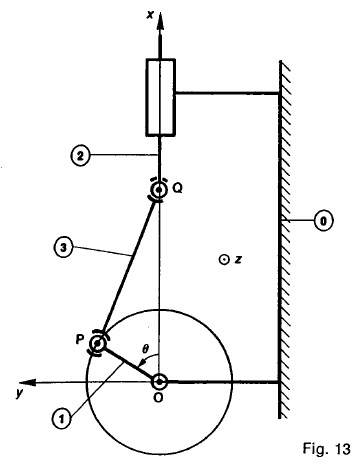
\includegraphics[scale=0.6]{png/bielle.png}
\end{center}

\subsubsection{Travail demandé}
\begin{enumerate}
\item Déterminer graphiquement la courbe représentative de la position du coulisseau par rapport au bâti en fonction de la position angulaire de la manivelle : $x(\theta)$ pour $\theta \in [0,2\pi]$.
\item En déduire par dérivation graphique la courbe représentative de la vitesse du coulisseau par rapport au bâti en fonction de la position angaire de la manivelle : $\theta'_t(\theta)=\frac{dx(\theta)}{dt}$ pour $\theta \in [0,2\pi]$.
\item En déduire par dérivation graphique la courbe représentative de l'accélération du coulisseau par rapport au bâti en fonction de la position angaire de la manivelle : $\theta''_t(\theta)=\frac{dx'_t(\theta)}{dt}$ pour $\theta \in [0,2\pi]$.
\end{enumerate}


\correction{ % Answer
\begin{center}
    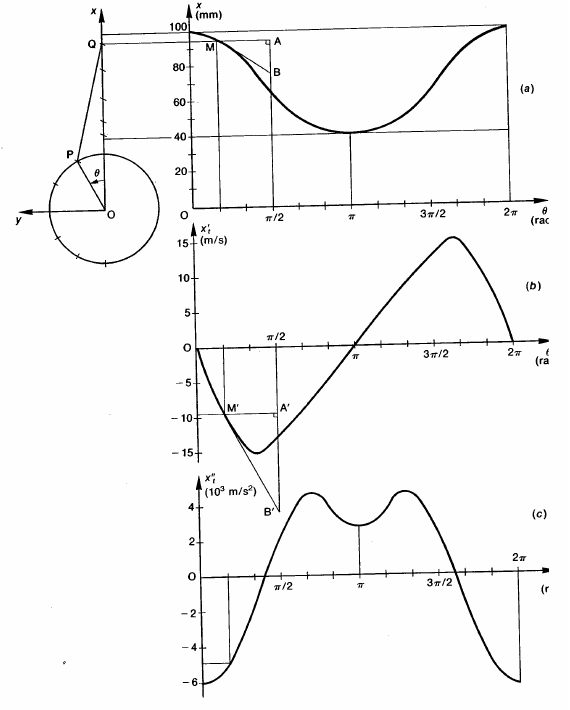
\includegraphics[scale=0.8]{png/bielle_correction.png}
\end{center}
}
\newpage
%--------------------------------------------

\exercice{Les KBOTS de l'ENS Cachan}

\begin{center}

\includegraphics[scale =0.1]{png/1_exo3.png}
\end{center}

Le club de robotique de l\rq{}ENS Cachan, [Kro]Bot, ont développé entre le mois de septembre et le mois de décembre des KBOTS.
Un KBOTS est un robot doté d'une architecture sandwich qui se déplace à l'aide de deux roues motrices.

\begin{figure}[h]
\centering
	\subfloat{%
		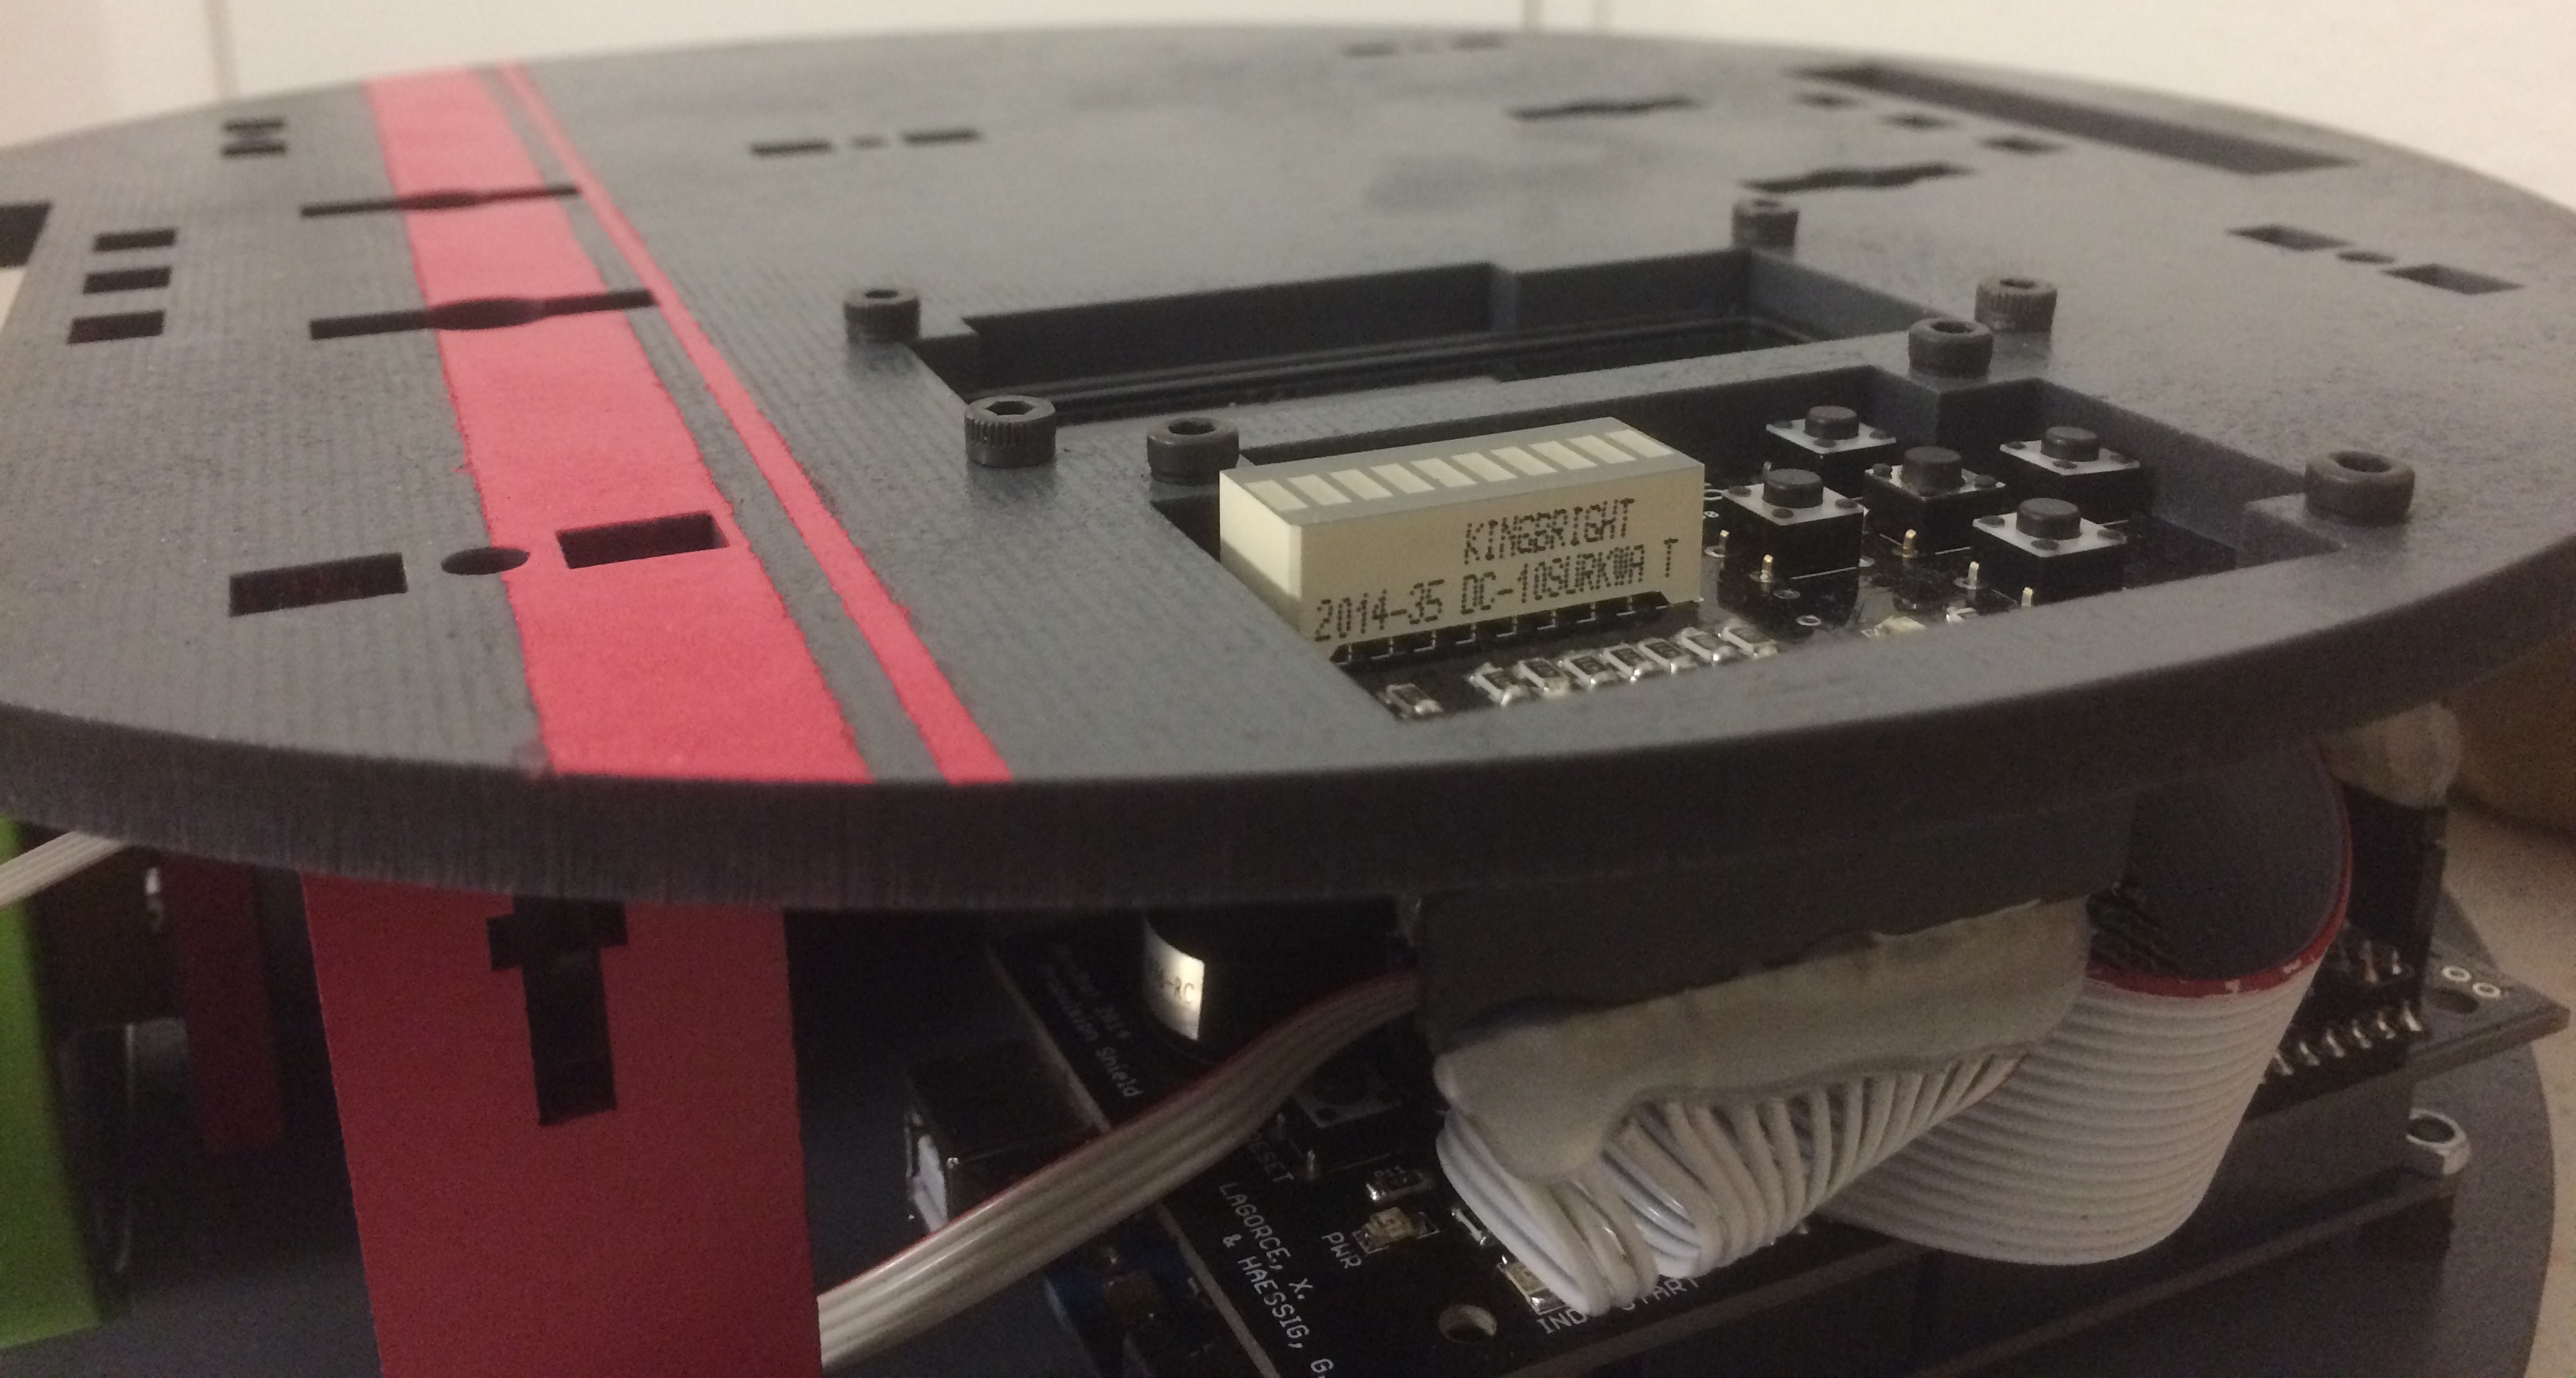
\includegraphics[height=3cm]{png/4_exo3.JPG}
	} 
	\subfloat{%
		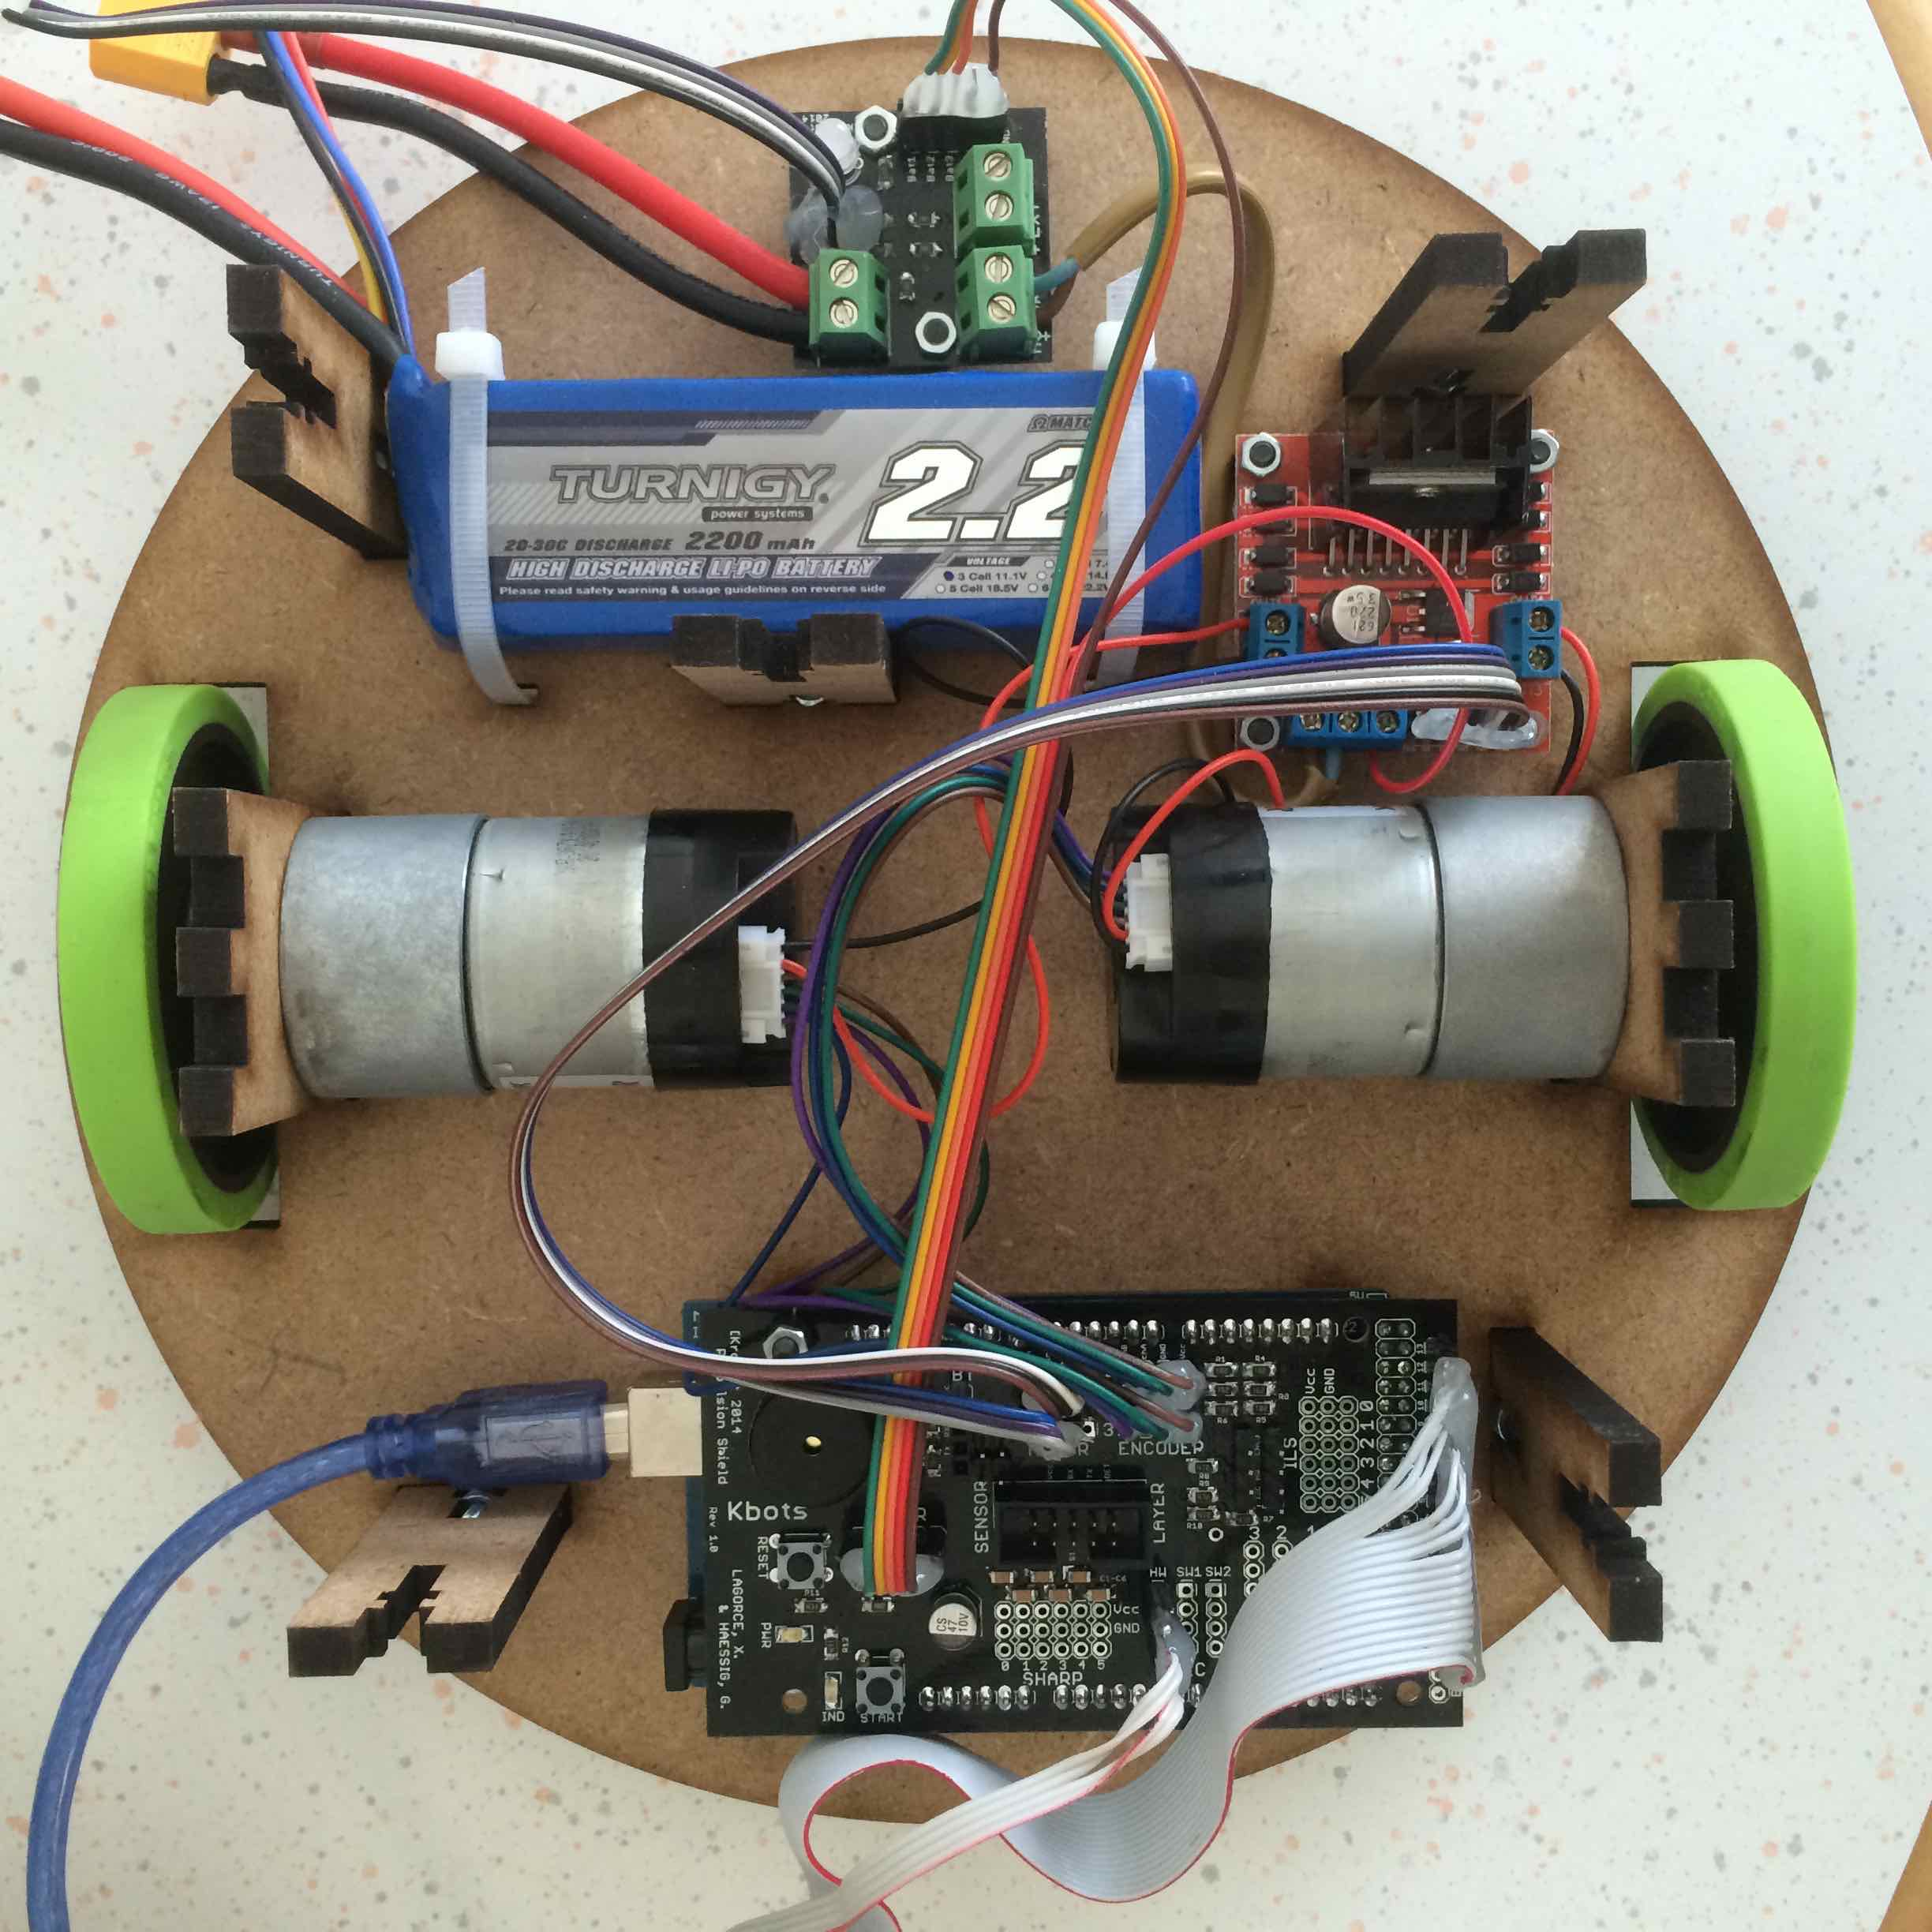
\includegraphics[height=3cm]{png/2_exo3.JPG}
	}
	\caption{Différentes prises de vues d'un KBOTS}
	\label{fig:default}
\end{figure}

L'asservissement, qui ne sera pas étudié durant la kholle, est un asservissement PI (proportionnel intégrale, cf. cours de SPÉ) en position sur chacune des roues du robots.
Il est donc indispensable d'établir les équations cinématique régissant le comportant des KBOTS avant de s'attaquer à la programmation de l'asservissement qui s'effectuera sur l'environnement $Arduino^{TM}$.

Le schéma cinématique d'un KBOTS vous est fourni :
\begin{center}
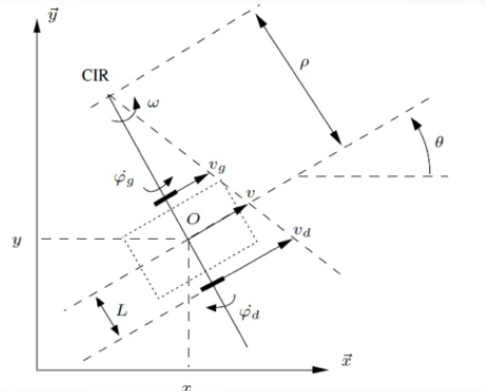
\includegraphics[scale =0.4]{png/3_exo3.png}
\end{center}

L'objectif sera donc de déterminer les relations liant les vitesses angulaires des roues aux vitesses de translation et de rotation du centre du robot.

\subsubsection{Travail demandé}
\begin{enumerate}
\item Déterminer la relation liant la vitesse angulaire d'une roue à la vitesse de translation de son moyeu.
\item Déterminer la relation liant la vitesse de translation du point $O$ aux vitesses de translation des moyeux.
\item Déterminer la relation liant la vitesse de rotation du point $O$ aux vitesses de translation des moyeux.
\item Déterminer les deux relations liant la vitesse de translation et la vitesse de rotation du point $O$ aux vitesses angulaires des roues.
\item Présenter les résultats des deux questions précédentes sous forme matricielle.
\end{enumerate}

\correction{ % Answer
\begin{enumerate}
\item \[v_d=-R\dot{\varphi_d}\]
\[v_g=R\dot{\varphi_g}\]
\item \[v=\frac{v_g+v_d}{2}\]
\item \[\omega=\frac{v_d-v_g}{2L}\]
\item \[v=R\frac{\dot{\varphi_g}-\dot{\varphi_d}}{2}\]
\[\omega=-R\frac{\dot{\varphi_d}+\dot{\varphi_g}}{2L}\]
\item \[\left( \begin{array}{c} v \\ \omega \end{array} \right)=-\frac{R}{2} \left( \begin{array}{cc} 1 & -1 \\
\frac{1}{L} & \frac{1}{L} \end{array} \right)
\left( \begin{array}{c} \dot{\varphi_d} \\ \dot{\varphi_g} \end{array} \right)\]

\end{enumerate}
}
\newpage

%--------------------------------------------

\exercice{Bras Manipulateur}
La figure ci-dessous représente un bras manipulateur permettant de déplacer des objets.\\
Ce mécanisme est constitué de :

\begin{itemize}
\item Un bâti $S_0$.
\item Un solide $S1$ entraîné en rotation par un moteur $M1$.
\item Un solide $S2$ entraîné en rotation par un moteur $M2$.
\item Un solide $S3$ entraîné en translation par un vérin $V1$.
\item Une pince située à l’extrémité du vérin permettant de saisir l’objet.
\end{itemize}

\vspace{1cm}
\begin{minipage}[c]{.45\linewidth}
	\begin{center}
    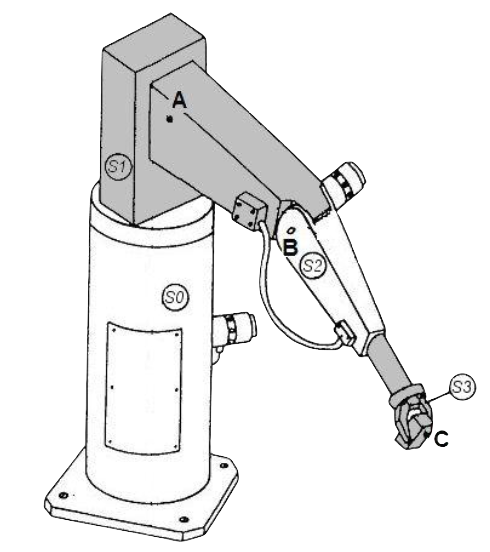
\includegraphics[scale=0.4]{png/1_exo2.png}
	\end{center}
\end{minipage}\hfill
\begin{minipage}[c]{.45\linewidth}
	\begin{center}
	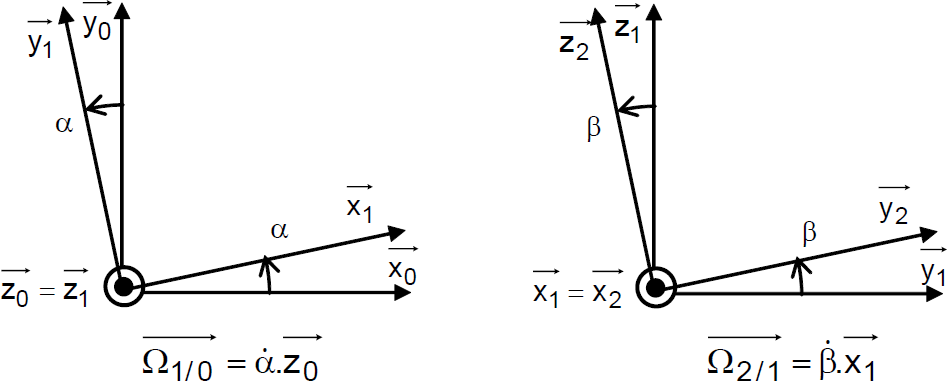
\includegraphics[scale=0.25]{png/parametrage.png}
	\end{center}
\end{minipage}
\vspace{1cm}

Remarques :
\begin{itemize}
\item $1/0$ : rotation d’axe $(A,\overrightarrow{z_0})$
\item $2/1$ : rotation d’axe $(B, \overrightarrow{x_1})$
\item $3/2$ : translation rectiligne de direction $\overrightarrow{z_2}$
\end{itemize}

On pose $\overrightarrow{AB} = a.\overrightarrow{y_1}$ (a étant une constante).

\subsubsection{Travail demandé}
\begin{enumerate}
\item Proposer un schéma cinématique du système.
\item Déterminer les trajectoires $T_{C\in3/2}$, $T_{C\in2/1}$ et $T_{C\in1/0}$.
\item Déterminer les vecteurs vitesses $\overrightarrow{V_{C\in3/2}}$, $\overrightarrow{V_{C\in2/1}}$, $\overrightarrow{V_{C\in1/0}}$ et $\overrightarrow{V_{C\in3/0}}$.
\item Déterminer le vecteur accélération $\overrightarrow{\Gamma_{C\in3/0}}$.
\end{enumerate}

\newpage

%--------------------------------------------

\exercice{Grue auxiliaire de chargement}

\subsubsection{Description}

\begin{center}
    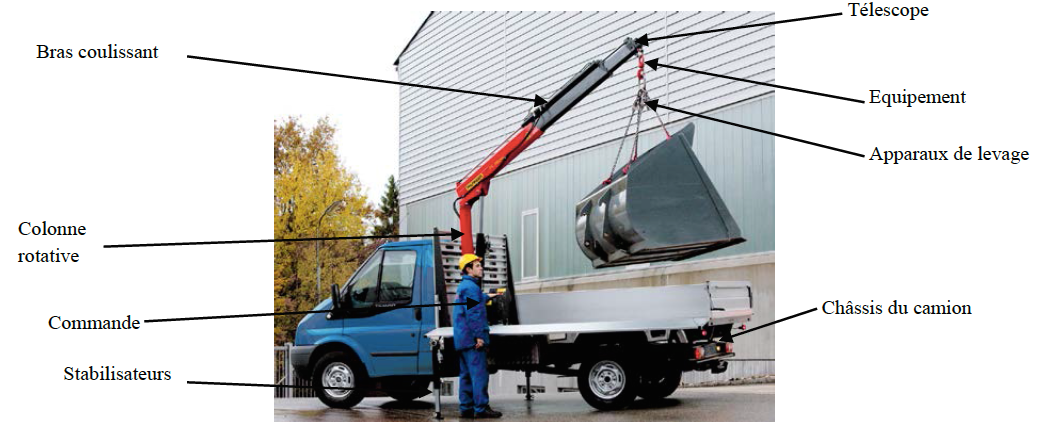
\includegraphics[scale=0.3]{png/1_exo8.png}
\end{center}

La dénomination "grues auxiliaires sur camion" correspond à des appareils de levage rapportés sur un châssis-porteur automoteur (camion) ou tracté (remorque de camion).\\
Le support, appelé châssis-porteur, ne doit pas pouvoir se déplacer en phase de travail, il est muni pour cela de vérins stabilisateurs. Les bras de levage sont généralement mus hydrauliquement. Ils peuvent être à montage fixe ou être partiellement amovibles.\\
Les grues auxiliaires comportent un socle, une colonne rotative, une flèche composée de bras articulés ou coulissants avec, dans certains cas, des rallonges qui peuvent être rapportées manuellement.\\
Les bras de flèche sont généralement du type repliable.\\

\subsubsection{Données géométriques}
$R_0(0,\overrightarrow{x_0},\overrightarrow{y_0},\overrightarrow{z_0})$ (en noir), 
$R_0(0,\overrightarrow{x_1},\overrightarrow{y_1},\overrightarrow{z_1})$ (en rouge), 
$R_0(A,\overrightarrow{x_2},\overrightarrow{y_2},\overrightarrow{z_2})$ (en vert), 
$R_0(B,\overrightarrow{x_2},\overrightarrow{y_2},\overrightarrow{z_2})$ (en bleu), 
avec $\overrightarrow{z_0}=\overrightarrow{z_1}$, et $\overrightarrow{x_1}=\overrightarrow{x_2}$\\
$\overrightarrow{OA}=h.\overrightarrow{z_0}$, $\overrightarrow{AB}=\lambda(t).\overrightarrow{y_2}$, $\overrightarrow{BC}=b.\overrightarrow{y_2}$, avec (b et h sont constants)

\begin{center}
    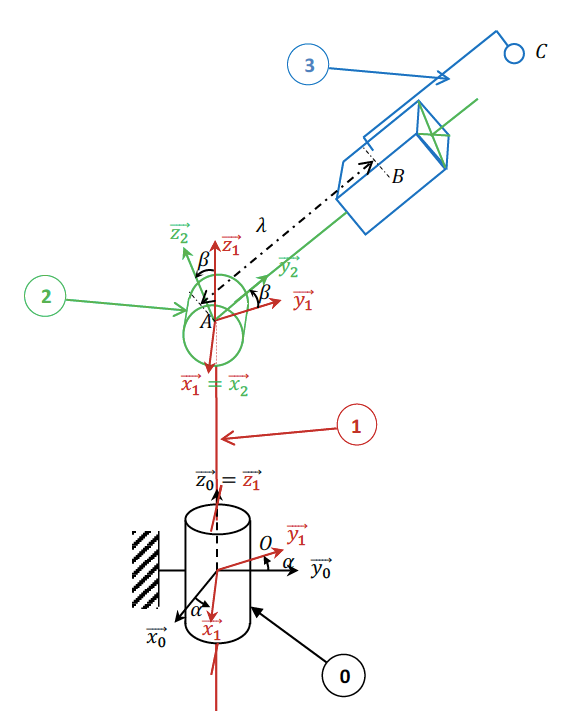
\includegraphics[scale=0.35]{png/2_exo8.png}
\end{center}

Le châssis $0$ et la colonne $1$ sont en liaison pivot d’axe $(0,\overrightarrow{z_1})$ : $\alpha(t)=(\overrightarrow{x_0},\overrightarrow{x_1})$\\
La colonne $1$ et le bras coulissant $2$ sont en liaison pivot d’axe $(0,\overrightarrow{x_1})$ : $\beta(t)=(\overrightarrow{z_1},\overrightarrow{z_2})$\\
Le bras coulissant $2$ et le télescope $3$ sont en liaison glissière d’axe $\overrightarrow{y_2}$ : $\overrightarrow{AB}=\lambda(t).\overrightarrow{y_2}$.\\

\subsubsection{Travail demandé}
\begin{enumerate}
\item \textbf{Position des différentes bases}\\
Mettre en place les figures de changement de bases relatives aux deux angles $\alpha$ et $\beta$.
\item \textbf{Position du point $C$}\\
Déterminer la position du point $C$ (appartenant à $3$) dans son mouvement par rapport à $0$.\\
Vous exprimerez le résultat dans le repère $R_0$. Le résultat doit être exprimé de manière concise.\\
Indiquer le lieu des points $C$ (dans son mouvement par rapport à $0$) lorsque les angles $\alpha$ et $\beta$ et la longueur $\lambda$ varient. (vous pouvez illustrez votre réponse d’une figure)
\item \textbf{Vecteur rotation $\overrightarrow{\Omega_{2/0}}$}\\
Déterminer le vecteur rotation $\overrightarrow{\Omega_{2/0}}$ du bras coulissant $2$ par rapport au châssis $0$.
\item \textbf{Relation sur les vitesses}\\
Donner la relation liant les vitesses : $\overrightarrow{V_{C\in2/1}}$, $\overrightarrow{V_{C\in3/0}}$, $\overrightarrow{V_{C\in1/0}}$ et $\overrightarrow{V_{C\in3/2}}$.
\item \textbf{Vitesse du point $C$ dans le mouvement de $2$ par rapport à $1$}\\
Déterminer la vitesse du point $C$ dans le mouvement de $2$ par rapport à $1$ : $\overrightarrow{V_{C\in2/1}}$.
\item \textbf{Vitesse du point $C$ dans le mouvement de $1$ par rapport à $0$}\\
Déterminer la vitesse du point $C$ dans le mouvement de $1$ par rapport à $0$ : $\overrightarrow{V_{C\in1/0}}$.
\item \textbf{Vitesse du point $C$ dans le mouvement de $3$ par rapport à $2$}\\
Déterminer la vitesse du point $C$ dans le mouvement de $3$ par rapport à $2$ : $\overrightarrow{V_{C\in3/2}}$.
\item \textbf{Vitesse du point $C$ dans le mouvement de $3$ par rapport à $0$}\\
Déterminer la vitesse du point $C$ dans le mouvement de $3$ par rapport à $0$ : $\overrightarrow{V_{C\in3/0}}$.
\item \textbf{Accélération du point $C$ dans le mouvement de $3$ par rapport à $0$}\\
Déterminer le vecteur accélération du point $C$ dans le mouvement de $3$ par rapport à $0$ : $\overrightarrow{\Gamma_{C\in3/0}}$
\end{enumerate}

\newpage

%--------------------------------------------

\exercice{Manège Spin fly}
\begin{center}
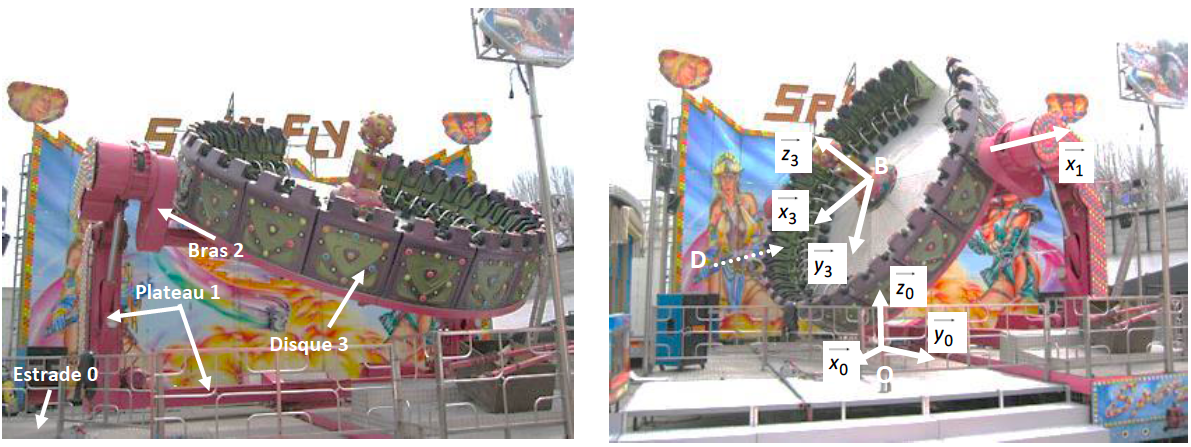
\includegraphics[scale=0.3]{png/manege.png}
\end{center}

\textit{On s'intéresse au manège Spin fly présent dans de nombreuses fêtes foraines (voir photos ci-dessus).}\\
\textbf{Objectif :} déterminer l'accélération subie par un client du manège, dans le but de vérifier que la limite supportable (sans inconfort) par l'homme de $2g$, ne soit pas dépassée.\\
Ce système est constitué de quatre solides :
\begin{itemize}
\item l'estrade $0$ (plancher), de repère $R_0(O,\overrightarrow{x_0},\overrightarrow{y_0},\overrightarrow{z_0})$, fixe par rapport à la terre telle que l'axe $(O,\overrightarrow{z_0})$ soit dirigé suivant la verticale ascendante ;
\item le plateau $1$, de repère associé $R_1(O,\overrightarrow{x_1},\overrightarrow{y_1},\overrightarrow{z_1})$, en mouvement de rotation d'axe $(O,\overrightarrow{z_0})$ par rapport à l'estrade $0$ tel que $\overrightarrow{z_0}=\overrightarrow{z_1}$ et $(\overrightarrow{x_0},\overrightarrow{x_1})=\Psi$ ;
\item le bras $2$, de repère associé $R_2(B,\overrightarrow{x_2},\overrightarrow{y_2},\overrightarrow{z_2})$, en mouvement de rotation d'axe $(B,\overrightarrow{x_1})$ par rapport au plateau $1$ tel que $\overrightarrow{OB}=b\overrightarrow{z_0}$ (avec $b$ constant), $\overrightarrow{x_1}=\overrightarrow{x_2}$ et $(\overrightarrow{y_1},\overrightarrow{y_2})=\theta$ ;
\item le disque $3$, de repère associé $R_3(B,\overrightarrow{x_3},\overrightarrow{y_3},\overrightarrow{z_3})$, en mouvement de rotation d'axe $(B,\overrightarrow{z_2})$ par rapport au bras $2$ tel que $\overrightarrow{z_2}=\overrightarrow{z_3}$ et $(\overrightarrow{x_2},\overrightarrow{x_3}=\phi$.\\
La position du point $D$ du disque $3$ est défini par : $\overrightarrow{BD}=c\overrightarrow{x_3}$ (avec $c$ constant).
\end{itemize}

\subsubsection{Travail demandé}
\begin{enumerate}
\item Réaliser les figures de changement de base illustrant les trois paramètres d'orientation. En déduire surs chaque figure, le vecteur rotation traduisant la figure.
\item Déterminer les trajectoires $T_{D \in 3/2}$, $T_{D \in 2/1}$, $T_{D \in 1/0}$ et $T_{D \in 3/0}$.
\item Déterminer les torseurs cinématiques $\nu(3/2)$, $\nu(2/1)$ et $\nu(1/0)$.
\item En déduire le torseur cinématique $\nu(3/0)$ au point $B$.
\item En déduire le torseur cinétique $\nu(3/0)$ au point $D$.
\item On se place dans le cas où le disque et le plateau tournent à vitesse constante : $\Psi=cte$ et $\phi=cte$.\\
Déterminer le vecteur accélération $\overrightarrow{\Gamma_{D \in 3/0}}$.
\end{enumerate}
\textit{La suite de l'étude consisterait à projeter ce vecteur dans une base unique afin de déterminer l'expression de sa norme\dots Puis, après application numérique, il serait possible de vérifer, si la limite supportable par l'homme ($2g$) est dépassée.}

\correction{
\begin{enumerate}
\item Figures de changement de base :
\begin{center}
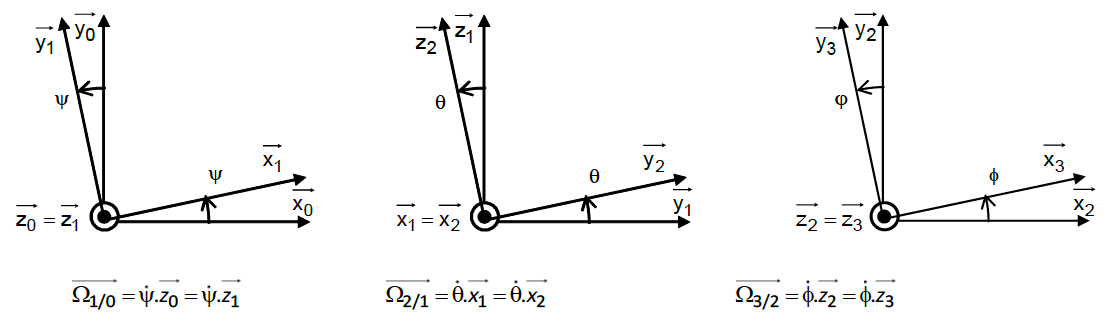
\includegraphics[scale=0.35]{png/manege_1.png}
\end{center}
\item Trajectoires :
\begin{itemize}
\item $T_{D \in 3/2}$ est un arc de cercle d'axe $(B,\overrightarrow{z_2})$, de centre $B$ et de rayon $[BD]$ ;
\item $T_{D \in 2/1}$ est un arc de cercle d'axe $(B,\overrightarrow{x_1})$, de centre $H_1$ (le projeté orthogonal de $D$ sur la droite $(B,\overrightarrow{x_1})$) et de rayon $[H_1D]$ ;
\item $T_{D \in 1/0}$ est un arc de cercle d'axe $(O,\overrightarrow{z_0})$, de centre $H_2$ (le projeté orthogonal de $D$ sur la droite $(O,\overrightarrow{z_0})$) et de rayon $[H_2D]$ ;
\item $T_{D \in 3/0}$ est une trajectoire quelconque.
\end{itemize}
\item Torseurs cinématiques :
\begin{center}
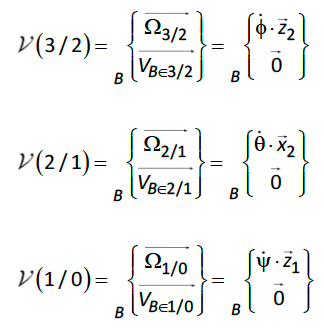
\includegraphics[scale=0.4]{png/manege_torseurs.png}
\end{center}
\item Avec des torseurs écrits au même point : $\nu(3/0)=\nu(3/2)+\nu(2/1)+\nu(1/0)$\\
Ainsi :
\[ \nu(3/0)=\left\{ \begin{array}{cc}
\dot{\Psi}\overrightarrow{z_1}+\dot{\theta}\overrightarrow{x_2}+\dot{\phi}\overrightarrow{z_2} \\ \overrightarrow{0} \end{array} \right\}_B \]
\item \[ \nu(3/0)=\left\{ \begin{array}{cc}
\overrightarrow{\Omega_{3/0}} \\ \overrightarrow{V_{D \in 3/0}} \end{array} \right\}_D \]
où \( \overrightarrow{V_{D \in 3/0}} = \overrightarrow{V_{B \in 3/0}}+\overrightarrow{DB}\wedge \overrightarrow{\Omega_{3/0}} \)
Ainsi :
\[ \nu(3/0)=\left\{ \begin{array}{cc}
\dot{\Psi}\overrightarrow{z_1}+\dot{\theta}\overrightarrow{x_2}+\dot{\phi}\overrightarrow{z_2} \\ c[(\dot{\Psi}cos(\theta)+\dot{\phi})\overrightarrow{y_3}-(\dot{\Psi}sin(\theta)cos(\phi)-\dot{\theta}sin(\phi))\overrightarrow{z_2}] \end{array} \right\}_D \]
\item \( \overrightarrow{\Gamma_{D \in 3/0}} = \frac{d \overrightarrow{V_{D \in 3/0}}}{dt}\) avec \( \overrightarrow{V_{D \in 3/0}} = c[(\dot{\Psi}cos(\theta)+\dot{\phi})\overrightarrow{y_3}-(\dot{\Psi}sin(\theta)cos(\phi)-\dot{\theta}sin(\phi))\overrightarrow{z_2}] \)
Ainsi :
\begin{center}
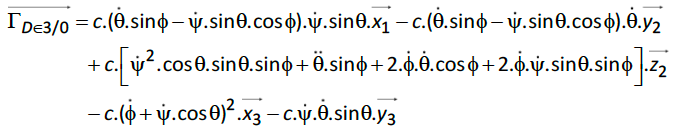
\includegraphics[scale=0.4]{png/acceleration_manege.png}
\end{center}
\end{enumerate}

\textbf{RAPPEL :} \( [\frac{d\overrightarrow{y_i}}{dt}]_j = \overrightarrow{\Omega_{i/j}} \wedge \overrightarrow{y_i} \)
}
\newpage

%--------------------------------------------
\exercice{Manège Magic Arms}
La manège Magic Arms dont la modélisation ainsi qu'un extrait de cahier des charges fonctionnel est composé d'une structure métallique d'environ $12\; m$ de haut avec deux bras mobiles. Les passagers s'assoient sur 39 pièces disposées sur une plate-forme tournante. Dès que tous les passagers sont assis et attachés, la nacelle tourne autour de son axe, le bras principal (bras 1) et le bras secondaires (bras 2), liés l'un à l'autre au début du cycle, commencent à tourner. Après 9 secondes, le maximum de hauteur est atteint et les deux bras se désindexent et se mettent à tourner indépendamment l'un de l'autre. Tous les mouvements sont pilotés par ordinateur. 

\begin{center}
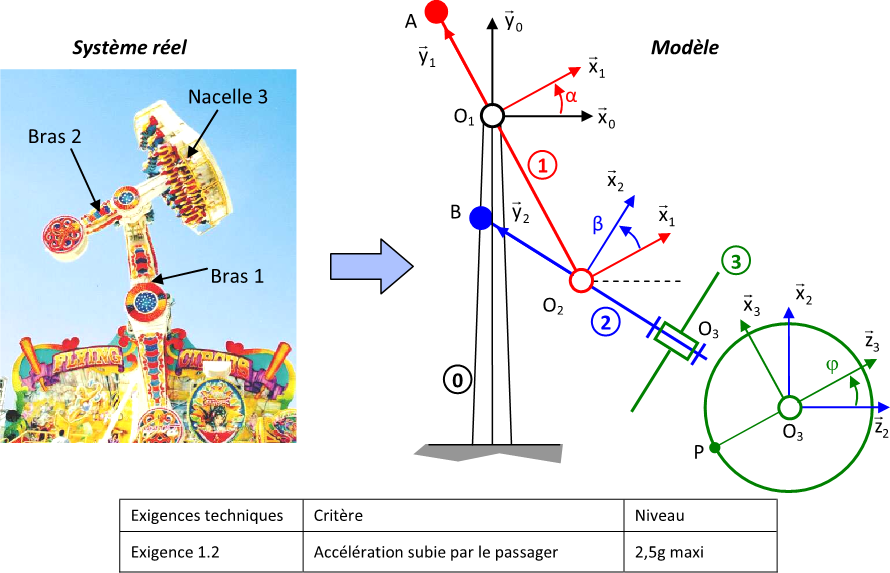
\includegraphics[width=.9\textwidth]{png/img1}
\end{center}

Le manège, schématisé ci-dessus, comporte :
\begin{itemize}
\item un bras principal 1 assimilé à une barre $AO_1O_2$. Il est en liaison pivot parfait d'axe $(O_1,\overrightarrow{z_1})$ caractérisée par le paramètre $\alpha$ avec le bâti 0. On pose $\overrightarrow{O_1O_2}=-l_1\overrightarrow{y_1}$;
\item un bras secondaire 2 assimilé à une barre $BO_2O_3$. Il est en liaison pivot parfait d'axe $(O_2,\overrightarrow{z_2})$ caractérisée par le paramètre $\beta$ avec le bras principal 1. On pose $\overrightarrow{O_2O_3}=-l_2\overrightarrow{y_2}$;
\item une nacelle 3 assimilée à un disque de centre $O_3$ et de rayon $R$. Elle est en liaison parfaite d'axe $(O_3,\overrightarrow{y_2})$ caractérisée par le paramètre $\varphi$ avec le bras 2. On s'intéresse plus particulièrement à un passager considéré comme un point matériel $P$ tel que $\overrightarrow{O_3P}=-R\overrightarrow{z_3}$.
\end{itemize}

\subsubsection{Travail demandé}
\begin{enumerate}
\item Construire les figures planes associées au schéma cinématique.
\item Calculer $\nu(1/0)$, $\nu(2/1)$ et $\nu(3/2)$ puis $\nu(3/0)$.
\item Calculer $\overrightarrow{\Gamma(0_3 \in 3/0)}$ puis $\overrightarrow{\Gamma(P \in 3/0)}$.
\end{enumerate}
\newpage

%--------------------------------------------
\exercice{Robot ramasseur de fruits}
On étudie un robot ramasseur de fruits. Il permet à un agriculteur de cueillir, de manière automatique, les fruits mûrs dans les arbres, et de les mettre dans un conteneur spécifique. 

Le bras 1 tourne autour de l'axe $(O_0,\overrightarrow{z_0})$ par rapport au bâti 0. Le bras 2 tourne autour de l'axe $(O_1,\overrightarrow{z_0})$ par rapport à 1. Le bras 3 tourner autour de l'axe $(O_2,\overrightarrow{z_0})$ par rapport à 2. On pose :
\begin{itemize}
\item $\overrightarrow{O_0O_1} = R\overrightarrow{x_1}$;
\item $\overrightarrow{O_1O_2} = R\overrightarrow{x_2}$;
\item $\overrightarrow{O_2M} = L\overrightarrow{x_3}$;
\end{itemize}

\begin{minipage}[c]{.47\linewidth}
\begin{center}
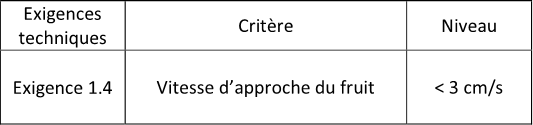
\includegraphics[width=.9\textwidth]{png/fig1}
\end{center}
\end{minipage}\hfill
\begin{minipage}[c]{.47\linewidth}
\begin{center}
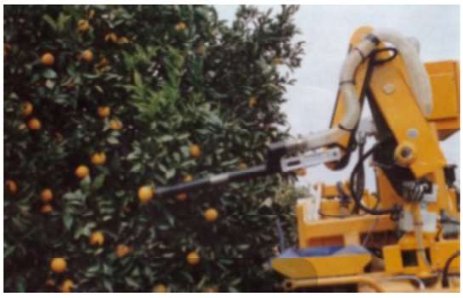
\includegraphics[width=.9\textwidth]{png/fig2}
\end{center}
\end{minipage}

\begin{center}
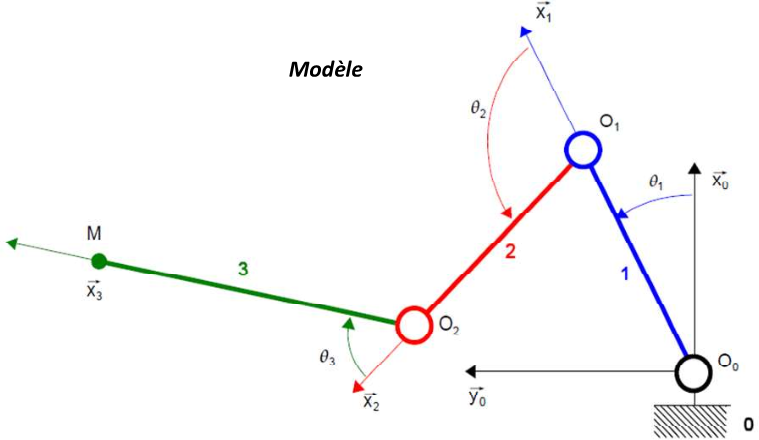
\includegraphics[width=.5\textwidth]{png/fig3}
\end{center}

\subsubsection{Travail demandé}
\begin{enumerate}
\item Construire les figures planes de repérage/paramétrage puis exprimer les vecteurs vitesse instantanée de rotation.
\item Déterminer $\nu(1/0)$, $\nu(2/1)$ et $\nu(3/2)$.
\item Déterminer $\nu(3/0)$.
\item Déterminer $\overrightarrow{\Gamma_{M(3/0)}}$.
\end{enumerate}

\correction{
\begin{enumerate}
\item Figures planes :
\begin{center}
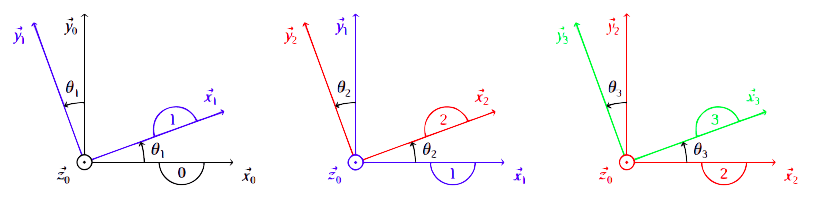
\includegraphics[scale=0.4]{png/figplanes.png}
\end{center}
$$
\overrightarrow{\Omega(1/0)}=\dot{\theta_1}\overrightarrow{z_0} \quad \quad
\overrightarrow{\Omega(2/1)}=\dot{\theta_2}\overrightarrow{z_0} \quad \quad
\overrightarrow{\Omega(3/2)}=\dot{\theta_3}\overrightarrow{z_0}
$$
\item \begin{align*}
\overrightarrow{V_{O_1 \in 1/0}} &= \overrightarrow{V_{O_0 \in 1/0}}+\overrightarrow{\Omega_{1/0}}\wedge\overrightarrow{0 O_1}\\
	&=\dot{\theta_1}\overrightarrow{z_{0}}\wedge R\overrightarrow{x_{1}}\\
\overrightarrow{V_{O_1 \in 1/0}})&=R\dot{\theta_1}\overrightarrow{y_{1}}
\end{align*}
\item \begin{align*}
\overrightarrow{V_{O_2 \in 2/0}}&=\overrightarrow{V_{O_1 \in 2/0}}+\overrightarrow{\Omega(2/0)}\wedge\overrightarrow{O_1 O_2}\\
	&=\overrightarrow{V_{O_1 \in 2/1}}+\overrightarrow{V_{O_1 \in 1/0}}+(\overrightarrow{\Omega(2/1)}+\overrightarrow{\Omega(1/0)})\wedge\overrightarrow{O_1 O_2}\\
	&=R\dot{\theta_1}\overrightarrow{y_{1}}+(\dot{\theta_2}+\dot{\theta_1})\overrightarrow{z_0}\wedge R\overrightarrow{x_2}\\
\overrightarrow{V_{O_2 \in 2/0}}&=R\dot{\theta_1}\overrightarrow{y_{1}}+R(\dot{\theta_2}+\dot{\theta_1})\overrightarrow{y_{2}}
\end{align*}
\item \begin{align*}
\overrightarrow{V_{M \in 3/0}}&=\overrightarrow{V_{O_2 \in 3/0}}+\overrightarrow{\Omega(3/0)}\wedge \overrightarrow{O_2 M}\\
	&=\overrightarrow{V_{O_2 \in 3/2}}+\overrightarrow{V_{O_2 \in 2/0}}+(\overrightarrow{\Omega(3/2)}+\overrightarrow{\Omega(2/1)}+\overrightarrow{\Omega(1/0)})\wedge \overrightarrow{O_2 M}\\
	&=R\dot{\theta_1}\overrightarrow{y_{1}}+R(\dot{\theta_2}+\dot{\theta_1})\overrightarrow{y_{2}}+(\dot{\theta_3}+\dot{\theta_2}+\dot{\theta_1})\overrightarrow{z_{0}}\wedge L \overrightarrow{x_{3}}\\
\overrightarrow{V_{M \in 3/0}}&=R\dot{\theta_1}\overrightarrow{y_{1}}+R(\dot{\theta_2}+\dot{\theta_1})\overrightarrow{y_{2}} +L(\dot{\theta_3}+\dot{\theta_2}+\dot{\theta_1})\overrightarrow{y_{3}}
\end{align*}
\end{enumerate}
}
\newpage

%--------------------------------------------
\exercice{Robot de manipulation}
Le système étudié est un robot industriel destiné à la manipulation de pièces lourdes. Ce robot a un structure en parallélogramme déformable qui lui permet de déplacer son poignet dans l'aire de travail.
\begin{center}
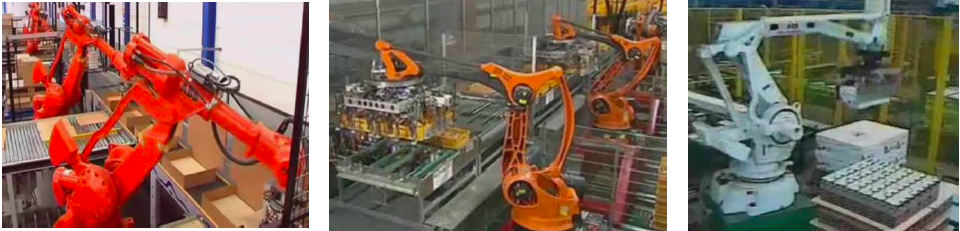
\includegraphics[scale=0.5]{png/robot_manipulateur.png}
\end{center}
On associe à chaque solide $i$ une base orthonormée directe $B_i(\overrightarrow{x_i},\overrightarrow{y_i},\overrightarrow{z})$
\begin{itemize}
\item Le mouvement de $1/0$ est une rotation d'axe $(A,\overrightarrow{z})$ ; on pose $\alpha=(\overrightarrow{x_0},\overrightarrow{x_1})$
\item Le mouvement de $2/0$ est une rotation d'axe $(A,\overrightarrow{z})$ ; on pose $\beta=(\overrightarrow{x_0},\overrightarrow{x_2})$
\item Le mouvement de $1/3$ est une rotation d'axe $(B,\overrightarrow{z})$
\item Le mouvement de $2/4$ est une rotation d'axe $(E,\overrightarrow{z})$
\item Le mouvement de $3/4$ est une rotation d'axe $(C,\overrightarrow{z})$
\end{itemize}
Par ailleurs : $\overrightarrow{AB}=L\overrightarrow{x_1}$, $\overrightarrow{EA}=D\overrightarrow{x_2}$, $\overrightarrow{CB}=D\overrightarrow{x_3}$, $\overrightarrow{BJ}=H\overrightarrow{x_3}$ et $\overrightarrow{EC}=L\overrightarrow{x_4}$

\begin{center}
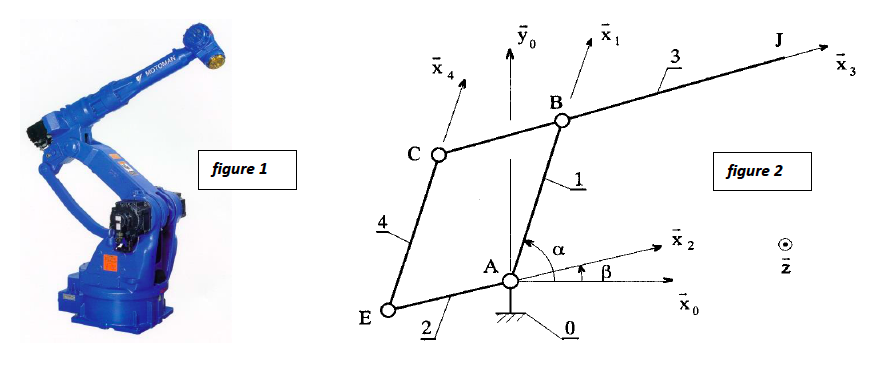
\includegraphics[scale=0.5]{png/robot_manip_cine.png}
\end{center}
Les mouvements du robot sont commandés par deux moteurs :
\begin{itemize}
\item Le solide $1$ a son mouvement de rotation par rapport à $0$ commandé par un moteur $M_1$ tel que : $\alpha \in [\frac{\pi}{3},\frac{2\pi}{3}]$ ;
\item Le solide $2$ a son mouvement de rotation par rapport à $0$ commandé par un moteur $M_2$ tel que : $\beta \in [-\frac{\pi}{4},\frac{\pi}{4}]$.
\end{itemize}
\subsubsection{Travail demandé}
\begin{enumerate}
\item Que peut-on dire sur les bases $B_1$, $B_2$, $B_3$ et $B_4$ ? En déduire les $2$ figures de changement de base définissant les $2$ paramètres d'orientation.
\item Déterminer les torseurs cinématiques $\nu(4/2)$ et $\nu(2/0)$.
\item En déduire le torseur cinématique $\nu(4/0)$ au point $E$.
\item Déterminer les torseurs cinématiques $\nu(3/1)$ et $\nu(1/0)$.
\item En déduire le torseur cinématique $\nu(3/0)$ au point $B$.
\item En déduire le vecteur vitesse $\overrightarrow{V_{J \in 3/0}}$.
\item Déderminer le vecteur accélération $\overrightarrow{\Gamma_{J \in 3/0}}$.
\item Déterminer la trajectoire $T_{J \in 3/0}$ lorsque le moteur $M_2$ est à l'arret et $\beta=0$.
\item Déterminer la trajectoire $T_{J \in 3/0}$ lorsque le moteur $M_1$ est à l'arret et $\alpha=\frac{\pi}{3}$.
\item Tracer sur une figure liée à $R_0$ dans laquelle se dépace le point $J$ lorsque $\alpha$ et $\beta$ varient dans les limites précédemment définies (les deux moteurs fonctionnent).
\end{enumerate}
\newpage


%--------------------------------------------

\exercice{Capsuleuse de bocaux}

\textbf{Objectif :} 
\begin{itemize}
\item Introduire la notion de vitesse de glissement
\item Établir la loi Entrée/Sortie lors d'une transmission de mouvement par contact ponctuel
\end{itemize}

\textbf{Objectif technologique:} 
\begin{itemize}
\item Diminuer l'usure dans les composants constituants la croix de Malte.
\item Valider que la vitesse de rotation du moteur empêche le basculement des bocaux.
\item Valider le choix du galet.
\end{itemize}

\subsubsection{Mise en situation}

\begin{minipage}[c]{.4\linewidth}
\begin{center}
 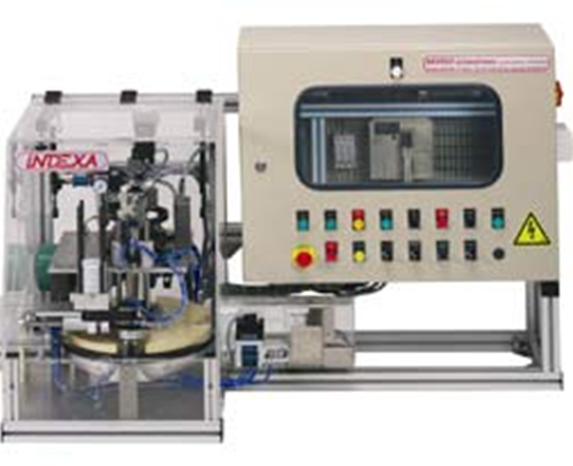
\includegraphics[width=\textwidth]{png/capsuleuse}
\end{center}

\end{minipage} \hfill
\begin{minipage}[c]{.55\linewidth}
Le conditionnement de nombreux produits alimentaires est réalisé dans des bocaux en verre fermés par des capsules vissées. La société RAVOUX, spécialisée dans le conditionnement, a créé ce prototype afin d'optimiser ses machines de production. Elle est donc équipée de nombreux capteurs permettant, via un ordinateur, d'optimiser les paramètres de production tels que qualité totale, production maximale, ...

Le système de laboratoire proposé s'insère dans une chaîne de conditionnement de produits alimentaires, entre l'unité de remplissage des bocaux et le poste d'étiquetage. Sa fonction principale est la «fermeture étanche de bocaux préalablement remplis de produits alimentaires»
\end{minipage}

\vspace{0.5cm}
\begin{minipage}[c]{.55\linewidth}
Ce système comprend plusieurs parties :
\begin{itemize}
\item un convoyeur linéaire d'alimentation des bocaux ;
\item un système électromécanique de transfert et d'indexation des bocaux (moto-réducteur, mécanisme à Croix de Malte, étoile de transfert) ;
\item un magasin de stockage des capsules ;
\item une partie opérative pneumatique de pose et de vissage des capsules - vérin V1, tête de vissage comprenant les vérins V2 et VR, ventouse et vacuostat (le vacuostat est une cellule permettant d'assurer la mise en dépression de la ventouse afin d'effectuer la préhension de la capsule) ;
\item un vérin de serrage des bocaux sous la tête de vissage ;
\item un convoyeur linéaire d'évacuation des bocaux ;
\item une partie commande par automate programmable Télémécanique TSX 37-10 64 entrées/sorties et un pupitre de commande.
\end{itemize}

\end{minipage} \hfill
\begin{minipage}[c]{.4\linewidth}
\begin{center}
 \includegraphics[width=\textwidth]{png/systeme3}
\end{center}
\end{minipage}

\vspace{0.5cm}
On s'intéresse ici au système de croix de Malte. Il permet d'obtenir une rotation discontinue à partir d'un mouvement de rotation continue. Ainsi, pendant que la croix de Malte ne tourne pas, le système peut agir sur la matière d'\oe{}uvre (flacon).

Lors de la rotation de la croix de Malte, la capsuleuse déplace deux flacons. Afin d'accroître la productivité, il faut diminuer la durée de cette phase. Cependant, si la croix de Malte tourne trop vite, les flacons basculent ce qui entraîne un mauvais fonctionnement du système. Ainsi, on désire que la \textbf{vitesse de la croix soit inférieure à 50 tours/minute}. 


\subsubsection{Modélisation sans galet}

\begin{minipage}[c]{.4\linewidth}
Afin de modéliser le système à croix de malte, on propose le schéma cinématique ci-contre. 


On note :
\begin{itemize}
\item $\mathcal{R}=\left( O,\overrightarrow{x_0},\overrightarrow{y_0},\overrightarrow{z_0}\right)$ le repère lié au bâti $S_0$. On note $\overrightarrow{OB}=-L\overrightarrow{x_0}$ avec $L = 145\; mm$;
\item $\mathcal{R}_1=\left( O,\overrightarrow{x_1},\overrightarrow{y_1},\overrightarrow{z_1}\right)$ le repère lié à l'arbre $S_1$. On pose $\overrightarrow{OA}=R\overrightarrow{y_1}$  avec $R =141\;mm$ et $\alpha = \left( \overrightarrow{x_0}, \overrightarrow{x_1}\right)$. L'arbre $S_1$ est lié au motoréducteur de la capsuleuse. On a : $\dot{\alpha} = 10\;tr/min$;
\item  $\mathcal{R}_2=\left( B,\overrightarrow{x_2},\overrightarrow{y_2},\overrightarrow{z_2}\right)$ le repère lié à l'arbre $S_2$. On pose $\overrightarrow{BA}=\lambda(t)\overrightarrow{x_2}$,  $\overrightarrow{AI}=r\overrightarrow{y_2}$ et $\beta = \left( \overrightarrow{x_0}, \overrightarrow{x_2}\right)$;
\end{itemize}


\end{minipage} \hfill
\begin{minipage}[c]{.55\linewidth}
\begin{center}
 \includegraphics[width=\textwidth]{png/schema1}
\end{center}
\end{minipage}

\subsubsection{Travail demandé}

\begin{enumerate}
\item Donner le paramétrage associé au schéma cinématique.
\item \'Etablir la loi entrée/sortie du système.
\item Donner une méthode permettant de valider la cahier des charges vis à vis de la vitesse de rotation de la croix de Malte.
\item Donner l'expression de $\overrightarrow{V(I,S_1/S_0)}$ et $\overrightarrow{\Omega(S_1/S_0)}$.
\item Donner l'expression de $\overrightarrow{V(I,S_2/S_0)}$ et $\overrightarrow{\Omega(S_2/S_0)}$
\item En déduire l'expression de $\overrightarrow{V(I,S_2/S_1)}$ dans la base $\mathcal{R}_2$. On donne $ \overrightarrow{x_1} 
=\cos(\alpha-\beta)\overrightarrow{x_2} + \sin(\alpha-\beta)\overrightarrow{y_2}$
\item D'après le paramétrage adopté, quelle est la direction du vecteur vitesse du solide $S_1$ par rapport à $S_2$ ? %Calculer ce vecteur comme dérivée du vecteur position. 
En utilisant les résultats de la question précédente, déduire une condition de fonctionnement du mécanisme.
\item $\overrightarrow{V(I,S_2/S_1)}\cdot\overrightarrow{x_2}$ est appelée \textbf{vitesse de glissement}. Quel problème technologique pose l'existence de cette vitesse ? Ce problème est-il pris en compte sur la capsuleuse ? Si oui, comment ? Si non, proposez une modification du système permettant la prise en compte de ce problème.
\end{enumerate}

\subsubsection{Modélisation avec galet}

\begin{minipage}[c]{.4\linewidth}
On considère maintenant l'existence d'un galet $S_3$ en bout de de l'arbre $S_1$. On fait l'hypothèse que le galet roule sans glisser dans le $S_2$. $S_3$ et $S_1$ sont en liaison pivot d'axe $\overrightarrow{z_0}$ et de centre $A$.

Le galet a un diamètre extérieur de $16\;mm$. D'après la documentation constructeur, la vitesse de rotation du galet ne doit pas dépasser les $5000\; tr/min$.
\end{minipage} \hfill
\begin{minipage}[c]{.55\linewidth}
\begin{center}
 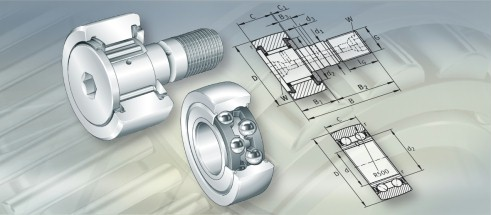
\includegraphics[width=\textwidth]{png/galet}
\end{center}
\end{minipage}

\begin{center}
 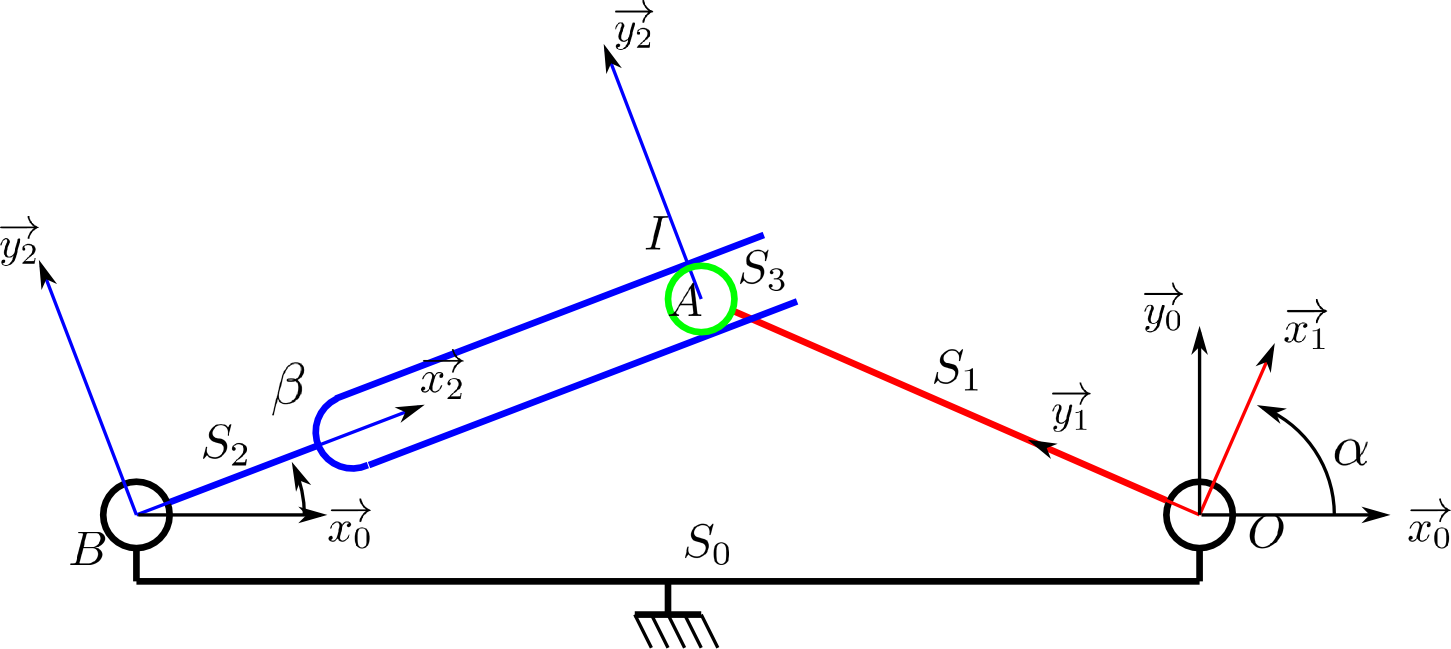
\includegraphics[width=.9\textwidth]{png/schema2}
\end{center}

\subsubsection{Travail demandé}

\begin{enumerate}
\item Quelle est la modification sur le paramétrage du système ?
\item Comment est-il possible de traduire l'hypothèse de \textbf{roulement} sans glissement ?
\item Calculer la vitesse de rotation du galet $\dot{\gamma}$ en commençant par exprimer $\overrightarrow{V(I,S_3/S_2)}$?
\item Indice : décomposer $\overrightarrow{V(I,S_3/S_2)}$ en fonction des mouvements connus.
\item Valider le choix du galet.
\end{enumerate}

\correction{
\textbf{Modélisation avec galet}
\begin{enumerate}
\item Paramétrage :
\begin{center}
 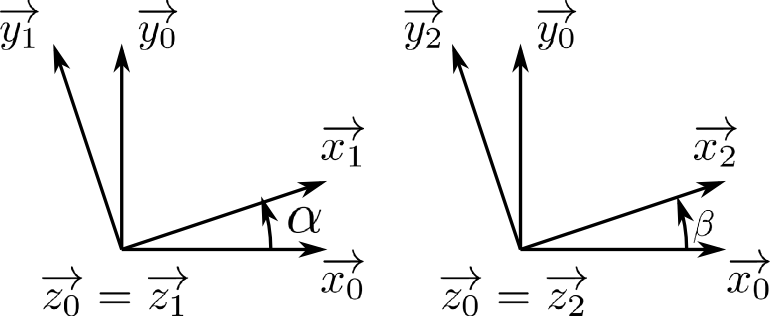
\includegraphics[width=.4\textwidth]{png/param1}
\end{center}
\item On a :
$$ \overrightarrow{OA} + \overrightarrow{AB} + \overrightarrow{BO} = \overrightarrow{0} \Longleftrightarrow 
R\overrightarrow{y_1} - \lambda(t)\overrightarrow{x_2} + L \overrightarrow{x_0} = \overrightarrow{0}
$$
En projetant sur $\overrightarrow{x_0}$ et $\overrightarrow{y_0}$ on a :
$$
\left\{
\begin{array}{l}
- R \sin \alpha(t) - \lambda(t) \cos\beta(t) + L = 0\\
R\cos\alpha(t) - \lambda(t)\sin \beta(t)=0
\end{array}
\right.
$$
Suivant le cas, on peut donc avoir $\alpha$ en fonction de $\beta$ ou $\lambda$ en fonction de $\alpha$ ou $\beta$ :
$$
\tan \beta = \dfrac{R\cos\alpha}{L-R\sin\alpha}
$$

$$
\lambda(t)^2 = R^2 + L^2 - 2RL \sin\alpha
$$
\item On peut calculer : 
$$
\dot{\beta} = \dfrac{R^2\dot{\alpha} - LR\dot{\alpha}\sin\alpha }{L^2-2RL\sin\alpha + R^2}
$$

Le tracé Excel permet de valider que la vitesse de rotation de la croix de Malte reste inférieure à 50 tours par minute.
\item $$\{\mathcal{V}(S_1/S_0)\} = 
\left\{
\begin{array}{l}
\overrightarrow{\Omega(S_1/S_0)} = \dot{\alpha}\overrightarrow{z_0} \\
\overrightarrow{V(O,S_1/S_0)} = \overrightarrow{0}
\end{array}
\right\}_O =
\left\{
\begin{array}{l}
\overrightarrow{\Omega(S_1/S_0)} = \dot{\alpha}\overrightarrow{z_0} \\
\overrightarrow{V(I,S_1/S_0)} = \overrightarrow{IO} \wedge \dot{\alpha}\overrightarrow{z_0}
\end{array}
\right\}_I
$$

$$
\overrightarrow{V(I,S_1/S_0)} =\left( -R\overrightarrow{y_1} - r \overrightarrow{y_2} \right) \wedge \dot{\alpha}\overrightarrow{z_0} =- R\dot{\alpha}\overrightarrow{x_1} - r\dot{\alpha}\overrightarrow{x_2}
$$
$$\{\mathcal{V}(S_1/S_0)\} = 
\left\{
\begin{array}{l}
\overrightarrow{\Omega(S_1/S_0)} = \dot{\alpha}\overrightarrow{z_0} \\
\overrightarrow{V(I,S_1/S_0)} = -R\dot{\alpha}\overrightarrow{x_1} - r\dot{\alpha}\overrightarrow{x_2}
\end{array}
\right\}_I
$$
\item $$\{\mathcal{V}(S_2/S_0)\} = 
\left\{
\begin{array}{l}
\overrightarrow{\Omega(S_2/S_0)} = \dot{\beta}\overrightarrow{z_0} \\
\overrightarrow{V(B,S_2/S_0)} = \overrightarrow{0}
\end{array}
\right\}_B =
\left\{
\begin{array}{l}
\overrightarrow{\Omega(S_2/S_0)} = \dot{\beta}\overrightarrow{z_0} \\
\overrightarrow{V(I,S_2/S_0)} = \overrightarrow{IB} \wedge \dot{\beta}\overrightarrow{z_0}
\end{array}
\right\}_I
$$
$$
\overrightarrow{V(I,S_2/S_0)} =\left( -\lambda(t)\overrightarrow{x_2} - r \overrightarrow{y_2} \right) \wedge \dot{\beta}\overrightarrow{z_0} = \lambda(t) \dot{\beta}\overrightarrow{y_2} - r\dot{\beta}\overrightarrow{x_2}
$$

$$\{\mathcal{V}(S_2/S_0)\} = 
\left\{
\begin{array}{l}
\overrightarrow{\Omega(S_2/S_0)} = \dot{\beta}\overrightarrow{z_0} \\
\overrightarrow{V(I,S_2/S_0)} = \lambda(t) \dot{\beta}\overrightarrow{y_2} - r\dot{\beta}\overrightarrow{x_2}
\end{array}
\right\}_I
$$
\item $$
\{ \mathcal{V}(S_2/S_1)\} = \{ \mathcal{V}(S_2/S_0)\} + \{ \mathcal{V}(S_0/S_1)\} 
\Longleftrightarrow \{ \mathcal{V}(S_2/S_1)\} = \{ \mathcal{V}(S_2/S_0)\} - \{ \mathcal{V}(S_1/S_0)\} 
$$
On a donc : 
$$
\{ \mathcal{V}(S_2/S_1)\} =
\left\{
\begin{array}{l}
\overrightarrow{\Omega(S_2/S_1)} = \overrightarrow{\Omega(S_2/S_0)} - \overrightarrow{\Omega(S_1/S_0)}  = \left(\dot{\beta}-\dot{\alpha} \right)\overrightarrow{z_0} \\
\overrightarrow{V(I,S_2/S_1)} = \overrightarrow{V(I,S_2/S_0)} - \overrightarrow{V(I,S_1/S_0)} 
=
 \lambda(t) \dot{\beta}\overrightarrow{y_2} - r\dot{\beta}\overrightarrow{x_2} +
 R\dot{\alpha}\overrightarrow{x_1} + r\dot{\alpha}\overrightarrow{x_2}
\end{array}
\right\}_I
$$

%$$
%\{ \mathcal{V}(S_2/S_1)\} =
%\left\{
%\begin{array}{l}
%\overrightarrow{\Omega(S_2/S_1)} = \left(\dot{\beta}-\dot{\alpha} \right)\overrightarrow{z_0} \\
%\overrightarrow{V(I,S_2/S_1)} =
 %-\lambda(t) \dot{\beta}\overrightarrow{x_2}  -  R\dot{\alpha}\overrightarrow{y_1} 
%\end{array}
%\right\}_I
%$$

$$ \overrightarrow{x_1} 
=\cos(\alpha-\beta)\overrightarrow{x_2} + \sin(\alpha-\beta)\overrightarrow{y_2}
$$
D'où :
$$
\overrightarrow{V(I,S_2/S_1)} =
 \lambda(t) \dot{\beta}\overrightarrow{y_2} - r\dot{\beta}\overrightarrow{x_2} +
 R\dot{\alpha}\cos(\alpha-\beta)\overrightarrow{x_2} +  R\dot{\alpha}\sin(\alpha-\beta)\overrightarrow{y_2} + r\dot{\alpha}\overrightarrow{x_2}$$
$$
\overrightarrow{V(I,S_2/S_1)} =\left[
\begin{array}{l}
- r\dot{\beta}+ R\dot{\alpha}\cos(\alpha-\beta) + r\dot{\alpha}\\
 \lambda(t) \dot{\beta}+  R\dot{\alpha}\sin(\alpha-\beta)\\
0\\
\end{array}
\right]_{\mathcal{R}_2}
$$
\item Nécessairement, la vitesse de glissement appartient au plan tangent au contact. On a donc :
$$
\left\{
\begin{array}{l}
- r\dot{\beta}+ R\dot{\alpha}\cos(\alpha-\beta)  +r\dot{\alpha} = \dot{\lambda}\\
 \lambda(t) \dot{\beta}+  R\dot{\alpha}\sin(\alpha-\beta)=0\\
\end{array}
\right.
$$
\item Cette vitesse de glissement provoque le frottement du doigt sur la croix de Malte. Ce frottement entraînant de l'usure, la capsuleuse de bocaux est équipée d'un galet.
\end{enumerate}

\vspace{0.5cm}
\textbf{Modélisation avec galet}
\begin{enumerate}
\item Un angle $\gamma$ correspondant à la rotation du galet sur lui même apparaît.
\item La vitesse est nulle entre le galet et la croix de Malte est nulle au point $I$ :
$$ 
\overrightarrow{V(I,S_3/S_2)} = \overrightarrow{0}
$$
\item Malgré l'introduction d'un nouveau composant, la position du point $I$ reste inchangée.

Il faut identifier le torseur $\{\mathcal{V}(S_3/S_2)\}$. 
Pour cela, la composition des vitesses donne :
$$
\{\mathcal{V}(S_3/S_2)\} = \{\mathcal{V}(S_3/S_1)\} + \{\mathcal{V}(S_1/S_2)\}  
$$


Au point $I$ on connaît déjà $\{\mathcal{V}(S_1/S_2)\}$.

Calculons $\{\mathcal{V}(S_3/S_1)\}$:

$$
\{\mathcal{V}(S_3/S_1)\}
= 
\left\{
\begin{array}{l}
\overrightarrow{\Omega(S_3/S_1)} = \dot{\gamma}\overrightarrow{z_0} \\
\overrightarrow{V(A,S_3/S_1)} = \overrightarrow{0}
\end{array}
\right\}_A =
\left\{
\begin{array}{l}
\overrightarrow{\Omega(S_3/S_1)} = \dot{\gamma}\overrightarrow{z_0} \\
\overrightarrow{V(I,S_3/S_1)} = \overrightarrow{IA} \wedge \dot{\gamma}\overrightarrow{z_0}
= -r\overrightarrow{y_2} \wedge \dot{\gamma}\overrightarrow{z_0} = -r \dot{\gamma}\overrightarrow{x_2}
\end{array}
\right\}_I
$$

On a donc :
$$
\overrightarrow{V(I,S_3/S_2)} = \overrightarrow{V(I,S_3/S_1)} + \overrightarrow{V(I,S_1/S_2)} 
$$
$$
\overrightarrow{V(I,S_3/S_2)} = -r \dot{\gamma}\overrightarrow{x_2} 
+\left(-r\dot{\beta}+ R\dot{\alpha}\cos(\alpha-\beta) + r\dot{\alpha}\right)\overrightarrow{x_2}
- \left(\lambda(t) \dot{\beta}+  R\dot{\alpha}\sin(\alpha-\beta)\right)\overrightarrow{y_2}
$$


$$
\overrightarrow{V(I,S_3/S_2)} =\left[ 
\begin{array}{l}
 -r \dot{\gamma}+\left(-r\dot{\beta}+ R\dot{\alpha}\cos(\alpha-\beta) + r\dot{\alpha}\right)\\
- \left(\lambda(t) \dot{\beta}+  R\dot{\alpha}\sin(\alpha-\beta)\right)\\
0\\
\end{array}
\right]_{\mathcal{R}_2}  
$$


%De même que précédemment, les solides étant indéformable, la projection de la vitesse sur $\overrightarrow{y_2}$ est nulle. 

D'après l'hypothèse de roulement sans glissement, on a :
$$ 
\overrightarrow{V(I,S_3/S_2)} = \overrightarrow{0} \Longrightarrow  \dot{\gamma}=-\dfrac{-r\dot{\beta}+ R\dot{\alpha}\cos(\alpha-\beta) + r\dot{\alpha}}{r}
$$
\item $$
 \dot{\gamma}=-\dfrac{-r\dot{\beta}+ R\dot{\alpha}\cos(\alpha-\beta) + r\dot{\alpha}}{r}
$$
\end{enumerate}
}
\newpage

%----------------------------------------------------------------------------------------
%	Schémas cinématiques
%----------------------------------------------------------------------------------------

\section{Schémas cinématiques}

%--------------------------------------------

\exercice{Un mélangeur}

Dessin d'un mélangeur
\begin{center}
    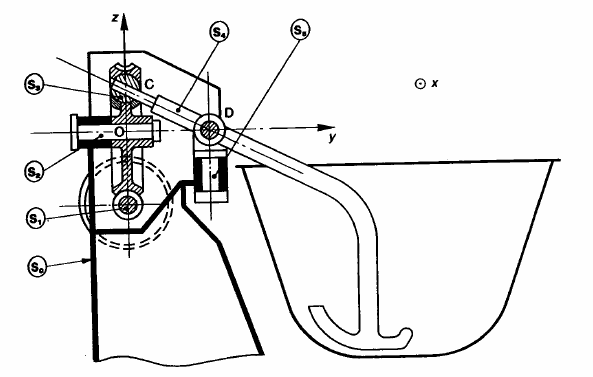
\includegraphics[scale=0.7]{png/melangeur.png}
\end{center}

\subsubsection{Travail demandé}
Établir le schéma cinématique paramétré de ce mécanisme.\\

\correction{ % Answer
\begin{center}
    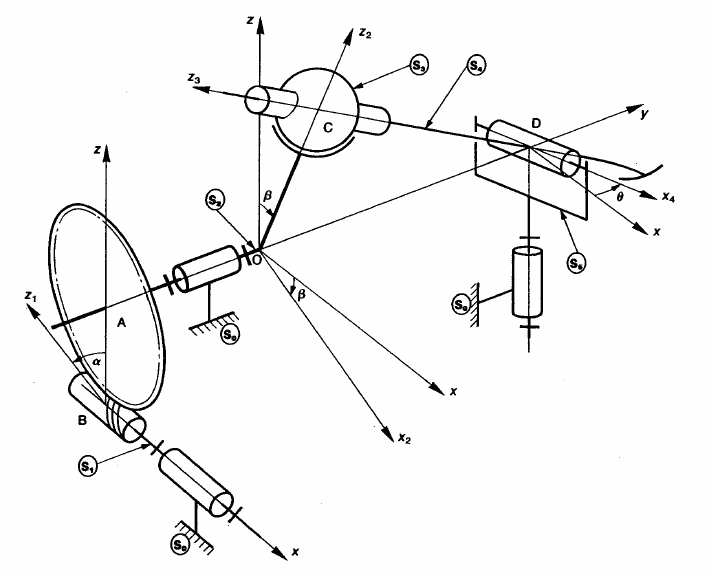
\includegraphics[scale=0.4]{png/melangeur_correction.png}
\end{center}
}
\newpage

%--------------------------------------------

\exercice{Guidage en rotation}

La figure $32$ représente le guidage en rotation du plateau $2$ dans le bâti $1$ d'un montage d'usinage, par l'intermédiare de l'arbre $3$.
\begin{center}
    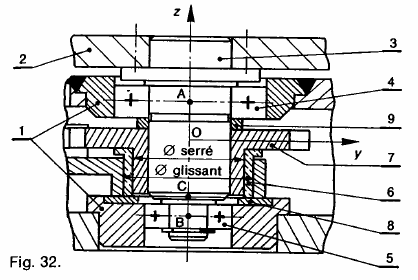
\includegraphics[scale=0.8]{png/plateau.png}
\end{center}

\subsubsection{Travail demandé}
\begin{enumerate}
\item Modéliser la liaison entre le plateau $2$ et l'arbre $3$.
\item Modéliser les liaisons entre l'arbre $3$ et le bâti $1$.
\item Concevoir le schéma cinématique du mécanisme.
\end{enumerate}

\correction{ % Answer
\begin{enumerate}
\item Le plateau est centré et épaulé sur l'arbre. Des vis représentées par les trait d'axe permettent de réaliser à partir de cette liaison pivot une laison encastrement.
\item Le guidage de l'arbre dans le bâti est réalisé à l'aide de trois liaisons élémentaires :
\begin{description}
\item L'angle de rotule du roulement à billes $4$ est supérieur à la déformation angulaire de l'arbre $3$. Cette laison est donc modélisable par une liaison linéique annulaire de centre $A$ et de direction $\vec{z}$.
\item En suivant le même raisonnement, la liaison entre l'arbre et le bâti réalisée par l'intermédiaire du roulement $5$ est modélisable par une liaison linéique annulaire de centre $B$ et de direction $\vec{z}$.
\end{description}
\item L'association de ces trois liaisons crée une liaison pivot unilatérale d'axe $(O,\vec{z})$ et dépend donc du sens des efforts.
\begin{center}
    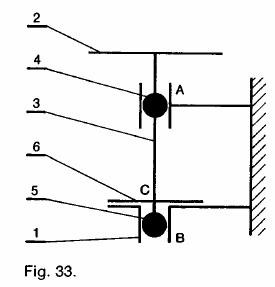
\includegraphics[scale=0.4]{png/plateau_correction.png}
\end{center}
\end{enumerate}
}
\newpage

%--------------------------------------------

\exercice{Actionneur de trieur à grains}

La figure $34$ représentante un mécanisme utilisé dans les silos à céréales permettant d'actionner un trieur à grains.
\begin{center}
    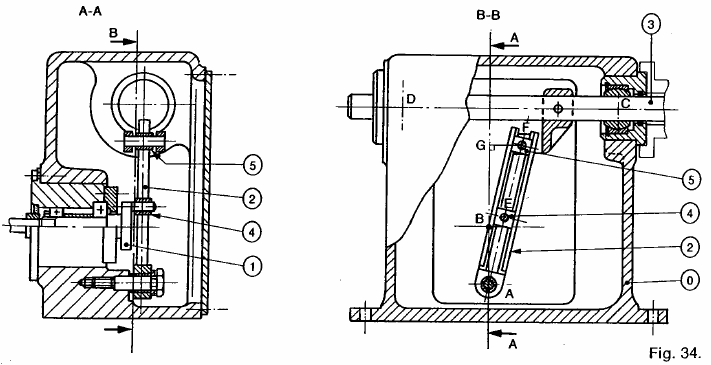
\includegraphics[scale=0.6]{png/trieur.png}
\end{center}

Un moteur électrique entraîne l'arbre $1$ d'un mouvement de rotation uniforme. Par l'intermédiaire de la bielle $2$, le coulisseau $3$ est animé d'un mouvement de translation alternatif.

\subsubsection{Travail demandé}
\begin{enumerate}
\item Modéliser les liaisons.
\item Concevoir les schémas cinématiques spatial et plan du mécanisme.
\item Paramétrer le schémacinématique plan en précisant les bases intermédiaires.
\item Établir la loi d'entrée-sortie, on pose : $AB=d$, $AG=h$ et $a$ le rayon de la manivelle $BE$.
\end{enumerate}

\correction{ % Answer
\begin{enumerate}
\item bâti $0$ - arbre $1$ : pivot\\
bâti $0$ - bielle $2$ : pivot\\
bielle $2$ - noix $4$ : glissière\\
noix $4$ - arbre $1$ : pivot glissant\\
bielle $2$ - noix $5$ : glissière\\
noix $5$ - arbre $3$ : pivot glissant\\
arbre $3$ - bâti $0$ en $C$ : linéique annulaire\\
arbre $3$ - bâti $0$ en $D$ : linéique annulaire
\item Schémas cinématiques :
\begin{center}
    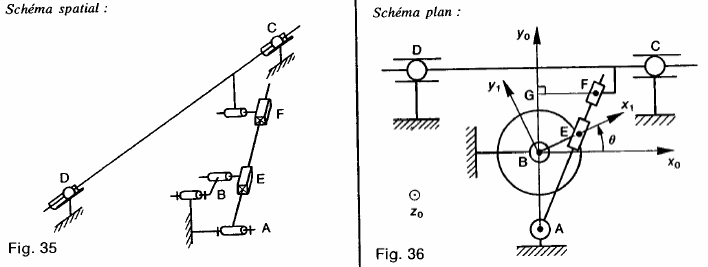
\includegraphics[scale=0.5]{png/trieur_correction.png}
\end{center}
\item Cf. schéma plan.
\item Loi d'entrée-sortie : $x=h.\frac{a.\cos(\theta)}{d+a.\sin(\theta)}$.
\end{enumerate}
}
\newpage

%--------------------------------------------

\exercice{Régulateur centrifuge du système DIRAVI CITROËN}

La figure $40$ représente le régulateur centrifuge du système DIRAVI CITROËN enntraîné à partir de la boîte de vitesses par flexible monté sur l'arbre $20$. Ce système permet de "durcir" la direction en fonction de la vitesse du véhicule.
\begin{center}
    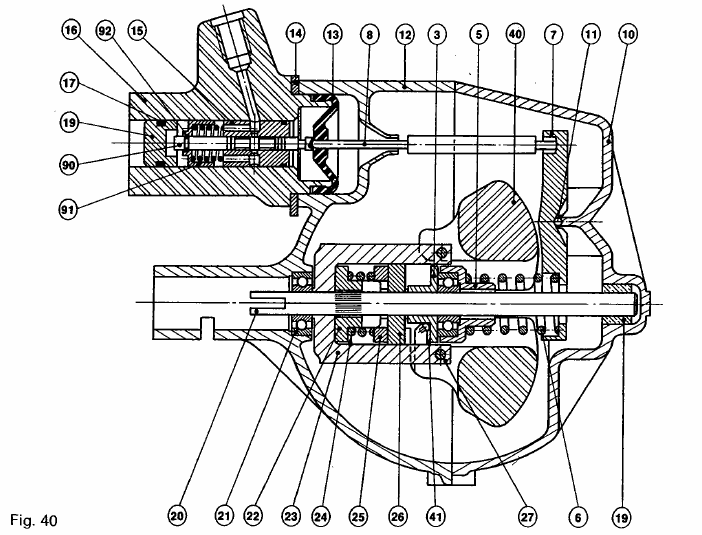
\includegraphics[scale=0.7]{png/citroen.png}
\end{center}

\subsubsection{Travail demandé}
\begin{enumerate}
\item Modéliser les liaisons (excepté le limiteur de couple constitué des pièces $22$, $23$, $24$, $25$, $26$ que l'on suppose liées à l'arbre $20$).
\item Tracer le schéma cinématique correspondant. Repèrer les ensembles de pièces cinématiquement liées par  leur numéro de classe d'équivalence. (exemple : ${90, 91, 92}$ sera repéré par $9$).
\item Paramètrer la position d'une masselotte $40$ par rapport au bâti.
\end{enumerate}
\newpage

%--------------------------------------------

\exercice{Le joint de OLDHAM}

Les figures $45$ et $46$ représentent un joint de OLDHAM permattent de transmettre une puissance entre deux arbres parallèles.
\begin{center}
    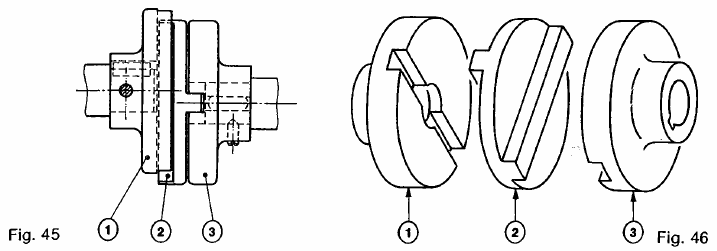
\includegraphics[scale=0.6]{png/joint.png}
\end{center}

\subsubsection{Travail demandé}
\begin{enumerate}
\item Modéliser les liaisons.
\item Concevoir un schéma cinématique paramétré.
\item Montrer que ce joint articulé est homocinétique.
\item Déterminer l'expression de la vitesse de translation de $1$/$2$ en fonction de $\dot{\theta}$ et $\theta$.
\item Déterminer l'expression de la vitesse de translation de $2$/$3$ en fonction de $\dot{\theta}$ et $\theta$.
\end{enumerate}

\correction{ % Answer
\begin{enumerate}
\item $1$-$2$ : liaisons glissières\\
$2$-$3$ : liaisons glissières
\item Schéma cinématique :
\begin{center}
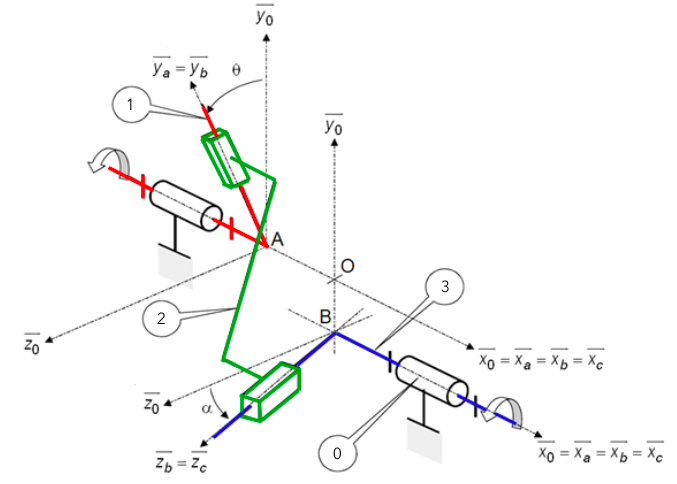
\includegraphics[scale=0.5]{png/oldham.png}
\end{center}
\item Fermeture cinématique : \[ \{V_{1/0}\}=\{V_{1/2}\}+\{V_{2/3}\}+\{V_{3/0}\} \]
Comme on souhaite $\dot{\alpha}=f(\dot{\theta},\theta)$, il ne faut pas faire apparaitre les paramètres indésirables des 2 liaisons glissières. C'est à dire écrire la composition des vecteurs vitesses de rotation en projection sur $\overrightarrow{X_0}$.
\[ \overrightarrow{\Omega_{1/0}}.\overrightarrow{X_0}=\overrightarrow{\Omega_{1/2}}.\overrightarrow{X_0}+\overrightarrow{\Omega_{2/3}}.\overrightarrow{X_0}+\overrightarrow{\Omega_{3/0}}.\overrightarrow{X_0} \]
Comme \( \overrightarrow{\Omega_{1/2}}.\overrightarrow{X_0}=0 \) et \( \overrightarrow{\Omega_{2/3}}.\overrightarrow{X_0}=0 \),
\[ \dot{\alpha}=\dot{\theta} \]
On en conclue que le joint de OLDHAM est homocinétique.
\item \[ \{V_{1/0}\}=\{V_{1/2}\}+\{V_{2/3}\}+\{V_{3/0}\} \]
Comme on souhaite $v_{y,P \in 1/2}=f(\theta,\dot{\theta})$, il ne faut pas faire apparaître les paramètres indésirables de la liaison glissière $2$/$3$ et de la liaison pivot $3$/$0$. C'est à dire écrire la composition des vecteurs vitesses au point $B$ en projection sur $\overrightarrow{y_b}$.
\[ \overrightarrow{V_{B \in 1/0}}.\overrightarrow{y_b}=\overrightarrow{V_{B \in 1/2}}.\overrightarrow{y_b}+\overrightarrow{V_{B \in 2/3}}.\overrightarrow{y_b}+\overrightarrow{V_{B \in 3/0}}.\overrightarrow{y_b} \]
\[ (\overrightarrow{V_{O \in 1/0}}+\overrightarrow{BO} \wedge \overrightarrow{\Omega_{1/0})}.\overrightarrow{y_b}=V_{y,P \in 1/2}+(V_{z,P \in 2/3}.\overrightarrow{z_b}).\overrightarrow{y_b}+0 \]
Comme $\overrightarrow{V_{O \in 1/0}}=0$ et $(V_{z,P \in 2/3}.\overrightarrow{z_b}).\overrightarrow{y_b}=0$,
\[ V_{y,P \in 1/2}=(f.\overrightarrow{y_0} \wedge \dot{\theta}.\overrightarrow{x_0}).\overrightarrow{y_b}=(-f.\dot{\theta}.\overrightarrow{z_0}).\overrightarrow{y_b}=-f.\dot{\theta}.\cos(\frac{\pi}{2}-\theta) \]
\[ V_{y,P \in 1/2}=-f.\dot{\theta}.\sin \theta \]
\item\[ \{V_{1/0}\}=\{V_{1/2}\}+\{V_{2/3}\}+\{V_{3/0}\} \]
Comme on souhaite $v_{z,P \in 2/3}=f(\theta,\dot{\theta})$, il ne faut pas faire apparaître les paramètres indésirables de la liaison glissière $1$/$2$ et de la liaison pivot $3$/$0$. C'est à dire écrire la composition des vecteurs vitesses au point $B$ en projection sur $\overrightarrow{z_b}$.
\[ \overrightarrow{V_{B \in 1/0}}.\overrightarrow{z_b}=\overrightarrow{V_{B \in 1/2}}.\overrightarrow{z_b}+\overrightarrow{V_{B \in 2/3}}.\overrightarrow{z_b}+\overrightarrow{V_{B \in 3/0}}.\overrightarrow{z_b} \]
\[ (\overrightarrow{V_{O \in 1/0}}+\overrightarrow{BO} \wedge \overrightarrow{\Omega_{1/0})}.\overrightarrow{z_b}=0+V_{z,P \in 2/3}+0 \]
Comme $\overrightarrow{V_{O \in 1/0}}=0$,
\[ V_{z,P \in 2/3}=(f.\overrightarrow{y_0} \wedge \dot{\theta}.\overrightarrow{x_0}).\overrightarrow{z_b}=(-f.\dot{\theta}.\overrightarrow{z_0}).\overrightarrow{z_b} \]
\[ V_{z,P \in 2/3}=-f.\dot{\theta}.\cos \theta \]
\end{enumerate}
}
\newpage

%----------------------------------------------------------------------------------------
%	Loi d'entrée-sortie
%----------------------------------------------------------------------------------------

\section{Loi d'entrée-sortie}

%--------------------------------------------

\exercice{Pompe hydraulique à pistons radiaux}
On s'intéresse au comportement cinématique du dispositif de transformation de mouvement par excentrique qui permet de transformer le mouvement de rotation continu de l'arbre d'entrée, sur lequel est fixé l'excentricité $1$, en mouvement de translation alternative du piston $2$.\\
Le comportement cinématique de ce système est modélisé par le schém cinématique ci-contre :

\begin{center}
    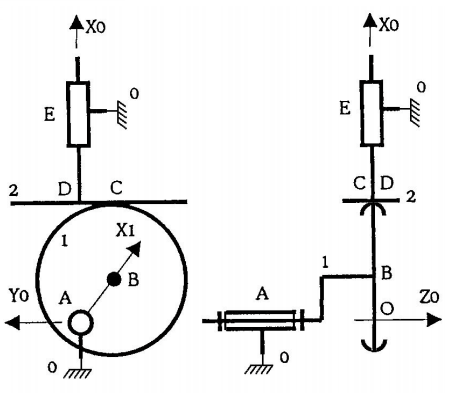
\includegraphics[scale=0.4]{png/1_exo1.png}
\end{center}

\subsubsection{Caractéristiques géométriques}
\[ |BC|=R \mbox{ et } |OB|=e \]

\subsubsection{Paramètres}
\[ (\overrightarrow{x_0},\overrightarrow{x_1})=\theta \mbox{, } \overrightarrow{OD}=X\overrightarrow{x_0} \mbox{ et } \overrightarrow{CD}=\lambda\overrightarrow{y_0} \]

\subsubsection{Travail demandé}
\begin{enumerate}
\item Tracer le graphe de liaison du système.
\item Donner les caractéristiques, le paramètre d'entrée et le paramètre de sortie du système.
\item Déterminer la loi d'entrée-sortie en position du système.
\item En déduire la vitesse du piston par rapport à celle du cylindre (loi E/S en vitesse).
\end{enumerate}

\correction{ % Answer
\begin{enumerate}
\item Graphe de liaison :
\begin{center}
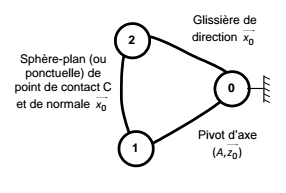
\includegraphics[scale=0.8]{png/pompe-graphe.png}
\end{center}
\item Caractéristiques : $R$ (rayon de l'excentrique) et $e$ (excentrique)\\
Paramètre d'entrée : $\theta$ (position angulaire de l'excentrique $1$ par rapport au bâti $O$.\\
Paramètre de sortie : $x$ (position linéaire du piston $2$ par rapport au bâti $O$).
\item Fermeture géométrique + projection sur $\overrightarrow{x_0}$ : \( x=e \cos \theta +R \)
\item Il suffit de dériver l'expression précédente : \( v=-e\dot{\theta} \sin \theta \)
\end{enumerate}
}
\newpage

%--------------------------------------------

\exercice{Fermeture géométrique, fermeture cinématique}

Le bras $(1)$ est lié au bâti $(0)$ par une liaison pivot d'axe $(O, \overrightarrow{z})$.\\
La roulette $(2)$, de rayon $r$, est liée au bras $(1)$ par une liaison pivot d'axe $(A,\overrightarrow{z})$.\\
Le plateau $(3)$ est lié au bâti par une liaison glissière de direction $\overrightarrow{y}$.
La roulette $(2)$ est en contact en $I$ avec le plateau $(3)$.

\begin{center}
    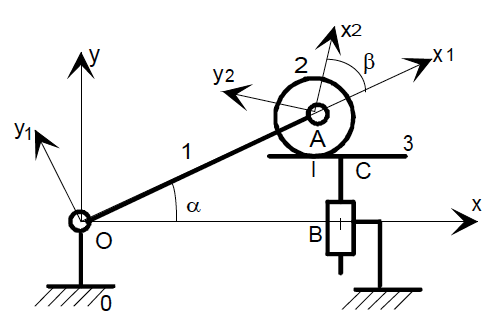
\includegraphics[scale=0.5]{png/1_exo5.png}
\end{center}

\begin{itemize}
\item $R(O,\overrightarrow{x},\overrightarrow{y},\overrightarrow{z})$ est associé à $(0)$.
\item $R_1(O,\overrightarrow{x_1},\overrightarrow{y_1},\overrightarrow{z_1}$ est associé à $(1)$.
\item $R_2(A,\overrightarrow{x_2},\overrightarrow{y_2},\overrightarrow{z_2})$ est associé à $(2)$.
\item $R3(C,\overrightarrow{x},\overrightarrow{y},\overrightarrow{z})$ est associé à $(3)$.
\end{itemize}

Données :\\
$\overrightarrow{OB}=b.\overrightarrow{x}$ et $\overrightarrow{OA}=a.\overrightarrow{x_1}$\\
Paramètres :\\
$\alpha=(\overrightarrow{x},\overrightarrow{x_1})$, $\beta=(\overrightarrow{x_1},\overrightarrow{x_2})$ et $\overrightarrow{BC}=\lambda.\overrightarrow{y}$

\subsubsection{Travail demandé}
\begin{enumerate}
\item Donner une relation entre $\alpha$ et $\lambda$ (effectuer une fermeture géométrique).
\item Donner la forme des torseurs cinématiques de $(1)$ par rapport à $(0)$, de $(2)$ par rapport à $(1)$ et de $(3)$ par rapport à $(0)$ à partir de l’analyse des liaisons. Identifier les paramètres cinématiques aux dérivées des paramètres géométriques.
\item Donner la condition cinématique associée au contact en $I$ (avec éventuellement glissement).
\item Déduire de la fermeture cinématique la relation entre $\dot{\alpha}$, $\dot{\lambda}$, $\alpha$, et les données géométriques. Vérifier ce résultat à l'aide de la première question.
\item En supposant qu'il y ait roulement sans glissement en $I$, donner la relation entre $\dot{\alpha}$, $\dot{\beta}$, $\alpha$ et les données géométriques.
\end{enumerate}

\correction{
\begin{center}
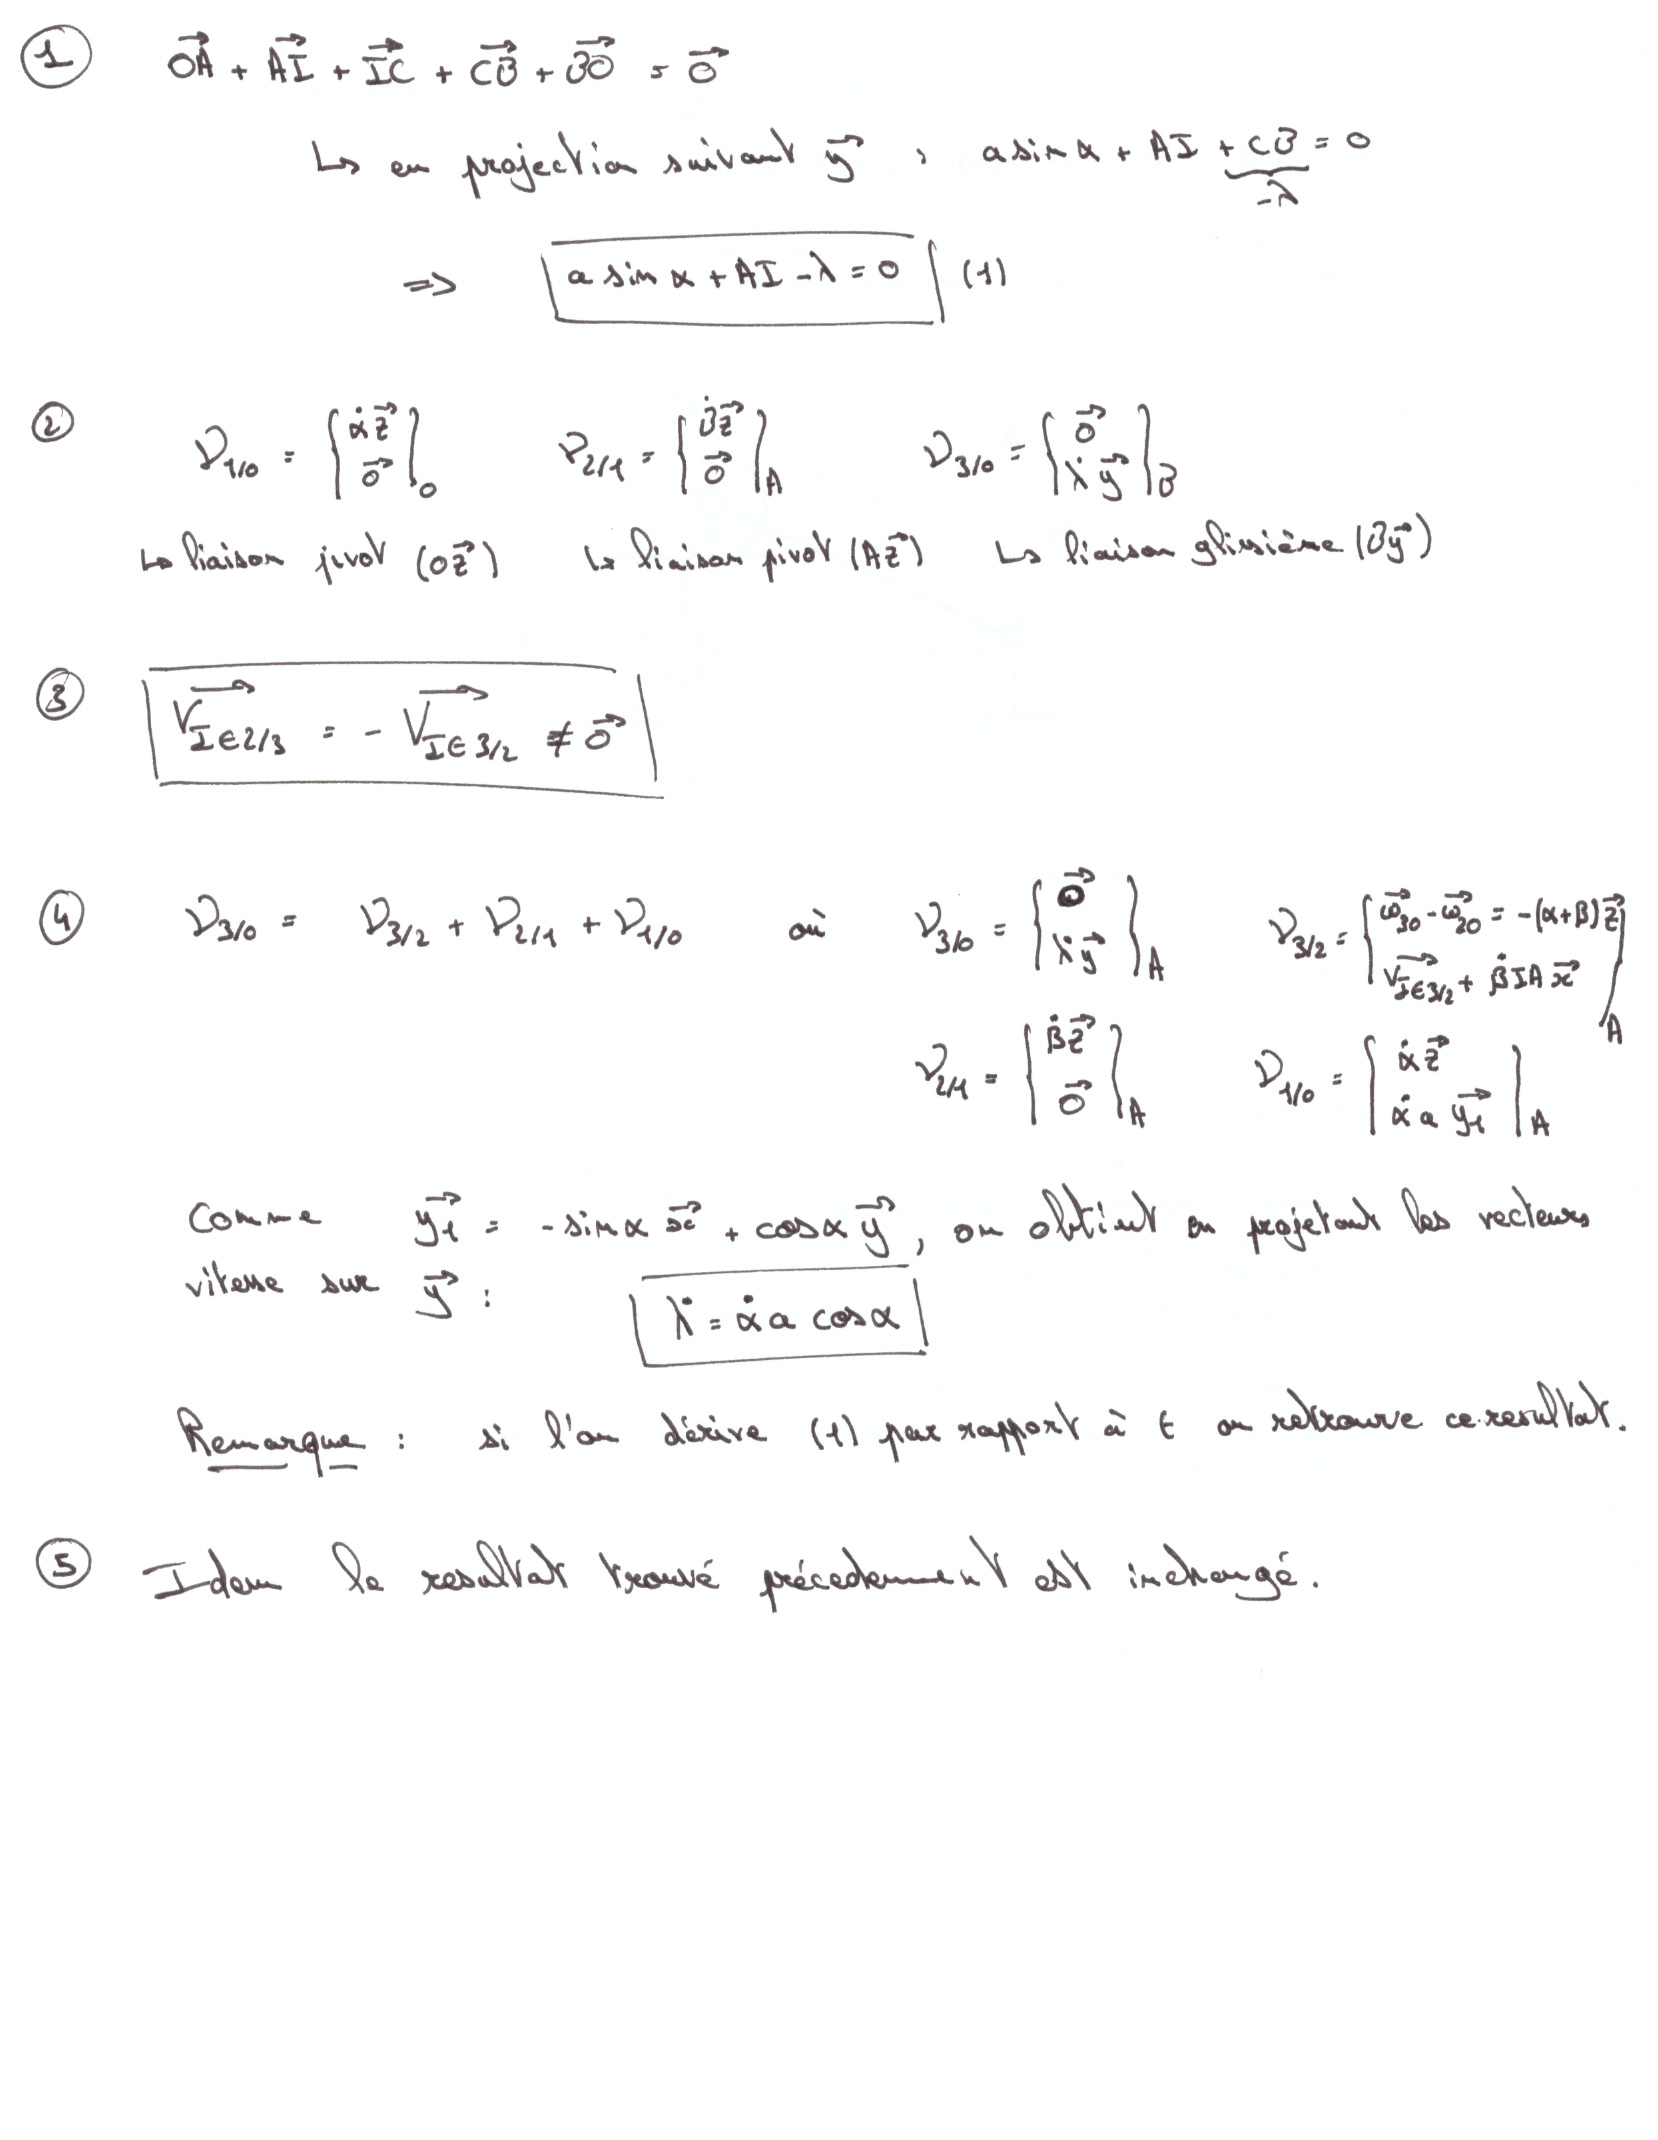
\includegraphics[scale=0.7]{png/correction-fermGEOfermCIN.png}
\end{center}
}
\newpage

%--------------------------------------------

\exercice{Mini-compresseur}

\begin{center}
    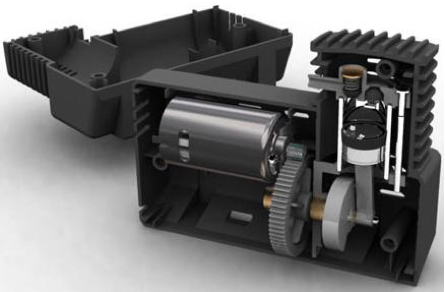
\includegraphics[scale=0.3]{png/1_exo0.png}
\end{center}

Ce compresseur est utilis\'e pour gonfler une roue de voiture, une roue de v\'elo, un ballon, un matelas... Il est vendu dans les r\'eseaux de grande distribution de types supermarch\'es. Son prix est inf\'erieur \`a 15 euros.\\
Son fonctionnement utilise le principe de transformation de mouvement de rotation continu (de la manivelle $2$ par rapport au b\^ati $1$) en un mouvement de translation alternatif (du piston $4$ par rapport au b\^ati $1$).\\
\\
NB : La transformation de mouvement dans le sens inverse (translation alternative en rotation continue) est utilis\'ee dans les moteurs thermiques (type automobiles).\\
\\
Sh\`ema cin\'ematique :
\begin{center}
    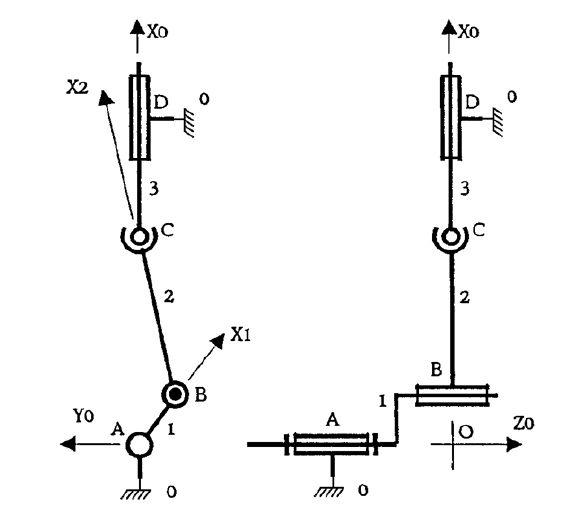
\includegraphics[scale=0.4]{png/2_exo0.png}
\end{center}

On s'int\'eresse maintenant seulement au dispositif "bielle-manielle" dans le cas g\'en\'eral.\\

\subsubsection{Travail demandé}
\begin{enumerate}
\item Donner le graphe de liaison de ce syst\`eme.
\item Donner les caract\'eristiques, le param\`etre d'entr\'ee et le param\`etre de sortie du syst\`eme.
\item D\'eterminer la loi d'entr\'ee-sortie en position du syst\`eme \`a l'aide d'une fermeture g\'eom\'etrique.
\item En d\'eduire la vitesse du piston par rapport au b\^ati (autrement dit la loi d'entr\'ee-sortie en vitesse).
\end{enumerate}

\correction{ % Answer
\begin{enumerate}
\item Graphe de liaison :
\begin{center}
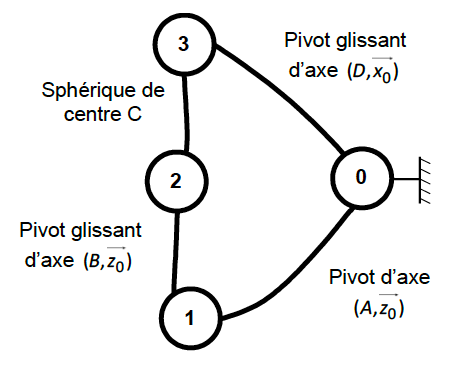
\includegraphics[scale=0.5]{png/mini-compresseur-graphe.png}
\end{center}
\item Paramètre d'entrée : $\theta_e=(\widehat{X_0,X_1})$ rotation de la bielle $1$ par rapport au bâti $0$.\\
Paramètre de sortie : $x=AC(t)$ déplacement du piston $3$.
Carcatéristiques : $L$ longueur de la bielle $2$ et $e$ longueur de la bielle $1$.
\item On pose $\beta=(\widehat{X_0,X_2})$\\
Fermmeture géométrique : \[\overrightarrow{OB}+\overrightarrow{BC}+\overrightarrow{CO}=\overrightarrow{0}\]
En projetant sur $\overrightarrow{x_0}$ et $\overrightarrow{y_0}$,
\[ \left\{ \begin{array}{rcl}
x=e\cos(\theta_e)+L\cos(\beta) \\ 
0=e\sin(\theta_e)+L\sin(\beta)
\end{array}\right. \]
On isole $\cos(\beta)$ et $\sin(\beta)$ pour les élever au carré et les sommer :
\[ (x-e\cos(\theta_e))^2+(-e\sin(\theta_e))^2=L^2 \]
\[ x=e \cos (\alpha) \pm \sqrt{L^2-(e \sin \alpha)^2} \]
Une longueur étant toujours positive, on en déduit : \( x=e \cos (\alpha) + \sqrt{L^2-(e \sin \alpha)^2} \)\\
\underline{Remarque :} Méthode plus rapide
\begin{center}
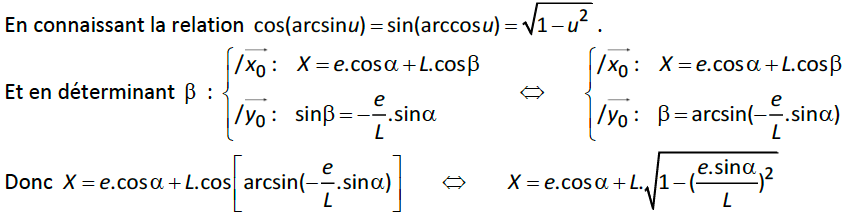
\includegraphics[scale=0.4]{png/methode-rapide.png}
\end{center}
\item Il suffit de dériver l'expression précédente. $$\dot{x}=-e\dot{\alpha}(\sin\alpha+\cos\alpha \frac{1}{\sqrt{L^{2}-(e\sin\alpha)^{2}}})$$
\end{enumerate}}
\newpage

%--------------------------------------------

\exercice{Joint de Cardan}

Un joint de Cardan permet de transmettre un mouvement de rotation entre deux arbres dont les axes sont concourants (mais pas forcément confondus).

\begin{center}
    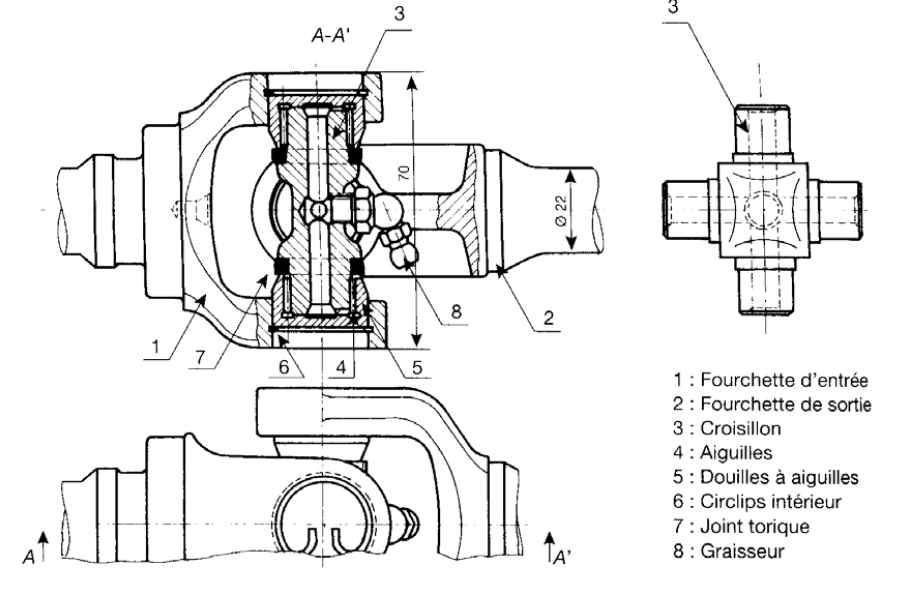
\includegraphics[scale=0.3]{png/1_exo6.png}
\end{center}

Les liaisons pivots entre les fourchettes d'entrée $(1)$, de sortie $(2)$ et le croisillon $(3)$ sont assurées par quatre douilles à aiguilles $(4 - 5)$. Le graisseur $(8)$ et les canalisations aménagées dans le croisillon en assurent la lubrification, le joint torique $(7)$ empêchant la sortie de la graisse et la pénétration d'impuretés.\\
Modélisation (les repères des pièces sont différents)

\begin{center}
    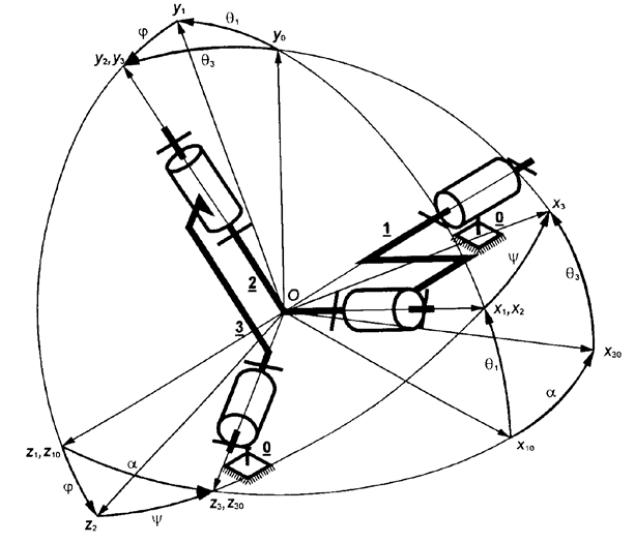
\includegraphics[scale=0.5]{png/2_exo6.png}
\end{center}

\begin{itemize}
\item $R_{10}(O,\overrightarrow{x_{10}},\overrightarrow{y_0},\overrightarrow{z_{10}})$ et $R_{30}(O,\overrightarrow{x_{30}},\overrightarrow{y_0},\overrightarrow{z_{30}})$ sont liés au bâti.
\item $R_1(O,\overrightarrow{x_1},\overrightarrow{y_1},\overrightarrow{z_1})$ est lié à la fourchette d'entrée $(1)$.
\item $R_3(O,\overrightarrow{x_3},\overrightarrow{y_3},\overrightarrow{z_3})$ est lié à la fourchette de sortie $(3)$.
\item $R_2(O,\overrightarrow{x_2},\overrightarrow{y_2},\overrightarrow{z_2})$ est lié au croisillon $(2)$.
\end{itemize}

Données :\\
$\alpha=(\overrightarrow{Z_{10}},\overrightarrow{Z_{30}})$ angle entre les axes des arbres d'entrée et sortie.\\
Paramètres :\\
$\theta_1=(\overrightarrow{x_{10}},\overrightarrow{x_1})$ et $\theta_3=(\overrightarrow{x_{30}},\overrightarrow{x_3})$

\subsubsection{Travail demandé}
\begin{enumerate}
\item Effectuer des figures planes faisant apparaître les angles $\alpha$, $\theta_1$ et $\theta_3$.
\item Donner la relation entre les paramètres de position $\theta_1$ et $\theta_3$. En déduire le rapport entre les vitesses angulaires des arbres d'entrée et de sortie ($\omega_1=\dot{\theta_1}$ et $\omega_3=\dot{\theta_3}$)\\

Les joints de Cardan sont souvent utilisés par deux en respectant les conditions suivantes :
\begin{itemize}
\item les arbres d'entrée et de sortie et l'arbre intermédiaire sont dans le même plan,
\item les axes des fourches liées à l'arbre intermédiaire sont parallèles,
\item les arbres de transmission sont parallèles (montage en $Z$), ou forment des angles égaux avec l'arbre intermédiaire (montage en $W$).
\end{itemize}

\begin{center}
    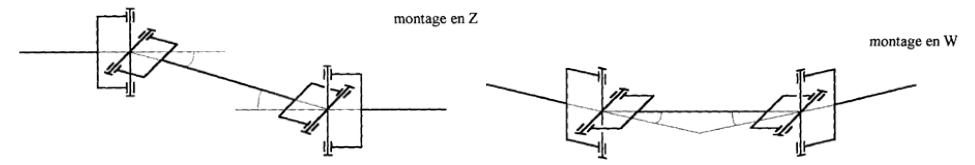
\includegraphics[scale=0.4]{png/3_exo6.png}
\end{center}

\item Quel est l'intérêt de ces montages ?
\end{enumerate}

\correction{ % Answer
\begin{enumerate}
\item Figures planes :
\begin{center}
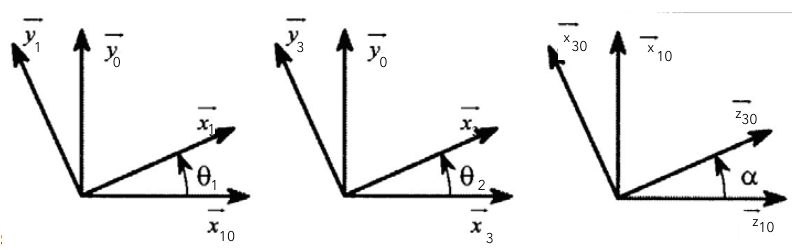
\includegraphics[scale=0.45]{png/fig_planes.png}
\end{center}
\item Comme \( \overrightarrow{x_1}.\overrightarrow{y_3}=\overrightarrow{0} \) avec :\\
\( \overrightarrow{x_1}=\cos(\theta_1)\overrightarrow{x_{10}}+\sin(\theta_1)\overrightarrow{y_0} \)\\
\( \overrightarrow{y_3}=-\sin(\theta_2)\overrightarrow{x_{30}}+\cos(\theta_2)\overrightarrow{y_0} \)\\
\( \overrightarrow{x_30}=\cos(\alpha)\overrightarrow{x_{10}}-\sin(\alpha)\overrightarrow{z_{10}} \)\\
On en déduit : \fbox{\( \tan(\theta_1)=\cos(\alpha)\tan(\theta_2) \)}\\
En dérivant l'expression : \fbox{\( (1+\tan(\theta_1)^2)\dot{\theta_1}=\cos(\alpha)(1+\tan(\theta_2)^2)\dot{\theta_2} \)}
\item Ces montages à deux joints de Cardan sont homocinétiques.
\end{enumerate}
}
\newpage

%----------------------------------------------------------------------------------------
%	Réducteurs
%----------------------------------------------------------------------------------------

\section{Réducteurs}

%--------------------------------------------

\exercice{Train épicycloïdal}

\begin{center}
    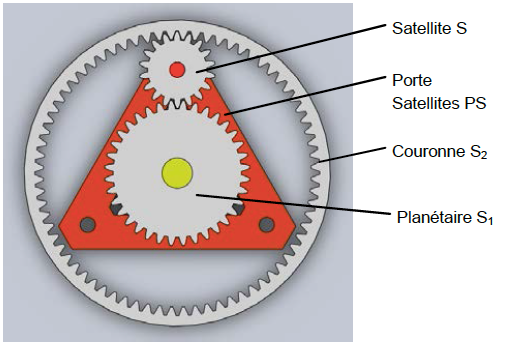
\includegraphics[scale=0.4]{png/2_exo7.png}
\end{center}

Le réducteur épicycloïdal est une solution technologique souvent utilisée. Elle permet d’obtenir un fort rapport de réduction dans un encombrement réduit avec un bon rendement (de l’ordre de 95\% pour un étage de réduction).\\
Le schéma cinématique ci-dessous représente un train épicycloïdal à axes parallèles constitué de cinq éléments : un planétaire $(S_1)$, un satellite $(S)$, un porte-satellite $(PS)$, une couronne $(S_2)$ et une pièce fixe $(S_0)$.\\
Le nombre de dents de la roue $S_1$ (resp. $S_2$ et $S$) est noté $Z_1$ (resp. $Z_2$ et $Z$).\\
Le repère $R_0 : (O,\overrightarrow{x_0},\overrightarrow{y_0},\overrightarrow{z_0})$ est lié à $(S_0)$. L'axe $(0,\overrightarrow{x})$, est parallèle à l'axe des roues dentées. Le repère $R : (O,\overrightarrow{x},\overrightarrow{y},\overrightarrow{z})$ est lié au porte satellite $(PS)$.\\
Il est noté : $\overrightarrow{\Omega}(S_1,R_0)=\omega_1.\overrightarrow{x}$, $\overrightarrow{\Omega}(S_2,R_0)=\omega_2.\overrightarrow{x}$, $\overrightarrow{\Omega}(PS,R_0)=\omega.\overrightarrow{x}$ et $\overrightarrow{\Omega}(S,PS)=\omega_s.\overrightarrow{x}$

\begin{center}
    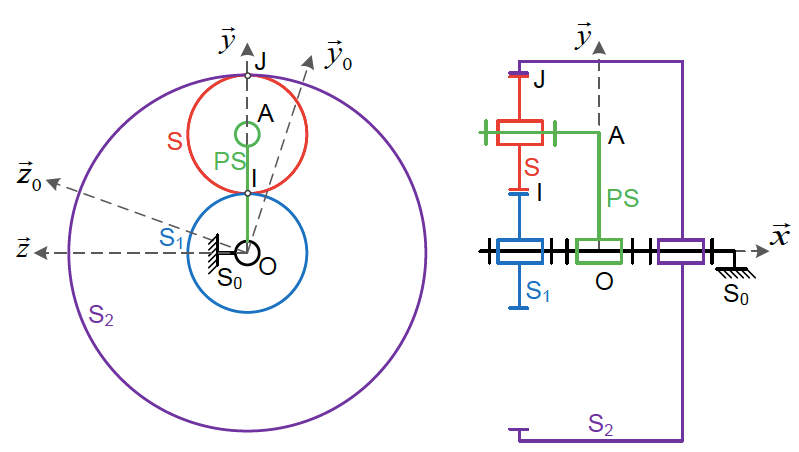
\includegraphics[scale=0.35]{png/1_exo7.png}
\end{center}

\subsubsection{Travail demandé}
\begin{enumerate}
\item Donner les éléments de réduction des torseurs cinématiques $V(S_1,R_0)$, $V(S_2,R_0)$, $V(PS,R_0)$ et $V(S,PS)$ en fonction de $\omega_1$, $\omega_2$, $\omega_s$ et $\omega$.
\item Donner les conditions de roulement sans glissement en $I$ et $J$.
\item Déterminer la relation entre $\omega_1$, $\omega_2$, $\omega$ et les nombre de dents $Z_1$ et $Z_2$ (écrire les équations issues de la fermeture des chaînes cinématiques).
\item Donner le rapport de réduction d’un réducteur constitué d’un train épicycloïdal où l’entrée est liée au planétaire, la sortie au porte-satellite et où la couronne est bloquée.
\end{enumerate}

\correction{
\begin{center}
\includegraphics[scale=0.7]{png/correction-Exo1-train-epi.png}
\end{center}
}
\newpage

%--------------------------------------------
\exercice{Étude cinétique du train épicycloidal double}
Soit le train épicycloidal suivant.
\begin{center}
\includegraphics[scale=0.35]{png/train-double.png}
\end{center}

\subsubsection{Travail demandé}
\begin{enumerate}
\item Le profil de denture étant en développante de cercle, exprimer le roulement sans glissement au point $A$ et $B$.
\item Exprimer la relation liant $\omega_{1/4}$ et $\omega_{4/2}$ par décomposition des vecteurs vitesses.
\item Même question pour la relation liant $\omega_{2/4}$ et $\omega_{4/3}$
\item En déduire la formule de Willis et celle de Ravignaux liant $\omega_1$, $\omega_3$ et $\omega_4$

\end{enumerate}
\correction{
\begin{enumerate}
\item Roulement sans glissement en $A$ et $B$ :
$$\overrightarrow{V_{A \in 1/2}}=\overrightarrow{0}$$ $$\overrightarrow{V_{B \in 2'/3}}=\overrightarrow{0}$$
\item En $A$, $\overrightarrow{V_{A \in 1/2}}=\overrightarrow{V_{A \in 1/4}}+\overrightarrow{V_{A \in 4/2}}=\overrightarrow{V_{O_1 \in 1/4}}+\overrightarrow{O_1A} \wedge \overrightarrow{\Omega_{1/4}}+\overrightarrow{V_{O_2 \in 4/2}}+\overrightarrow{O_2A} \wedge \overrightarrow{\Omega_{4/2}}=\overrightarrow{0}$\\
d'où $$ R_1 \omega_{1/4}-R_2 \omega_{4/2}=0$$
\item En $B$, $\overrightarrow{V_{B \in 2/3}}=\overrightarrow{V_{B \in 2/4}}+\overrightarrow{V_{A \in 4/3}}=\overrightarrow{V_{O_2 \in 2/4}}+\overrightarrow{O_2B} \wedge \overrightarrow{\Omega_{2/4}}+\overrightarrow{V_{O_3 \in 4/3}}+\overrightarrow{O_3B} \wedge \overrightarrow{\Omega_{4/3}}=\overrightarrow{0}$\\
d'où $$ R_{2'} \omega_{2/4}-R_3 \omega_{4/3}=0$$
\item Formule de Willis :
$$ \frac{\omega_1 -\omega_4}{\omega_3 -\omega_4}=-\frac{R_2R_3}{R_{2'}R_1}=\lambda$$
Formule de Ravignaux :
$$\omega_1-\lambda \omega_3+(\lambda-1)\omega_4=0$$
\end{enumerate}

\textbf{Remarque :}\\
On constate que si l'on se place dans le repère lié au porte satellites, tous les axes sont fixes. C'est pourquoi, nous décomposons les vecteurs vitesses en passant par le porte satellites.
}
\newpage

%--------------------------------------------
\exercice{Train épicycloïdal double}

\begin{center}
    \includegraphics[scale=0.5]{png/1_exo10.png}
\end{center}

Dans le train épicycloïdal représenté ci–dessus, le satellite ${(2),(3)}$ roule sans glisser à l'intérieur de la couronne $(4)$ liée à l'arbre d'entrée $(E)$ et sur la route d'entrée $(1)$ fixe. Le porte satellite $(5)$ est lié à l'arbre de sortie $(S)$.

\subsubsection{Travail demandé}
\begin{enumerate}
\item Donner l'expression de la loi d'entrée-sortie du système, $\frac{\omega_{50}}{\omega_{40}}=\frac{\omega_s}{\omega_e}$, en fonction de $R_1$, $R_4$ et $R_5$.
\item Donner les expressions des torseurs cinématiques en $A$ du mouvement de $(4)$ et de ${(2),(3)}$ par rapport à $(0)$ (en fonction de $\omega_{40}$, $R_1$, $R_4$ et $R_5$).
\end{enumerate}

\correction{
\begin{enumerate}
\item Rappelons : $$\frac{\omega_{s/PS}}{\omega_{e/PS}}=(-1)^p \frac{\Pi R_{menantes}}{\Pi R_{menees}}$$
On établit à l'aide cette formule :
$$\frac{\omega_{3/5}}{\omega_{4/5}}=\frac{R_3}{R_4} \text{ et }
\frac{\omega_{1/5}}{\omega_{2/5}}=-\frac{R_1}{R_2}$$
Notons aussi que $\omega_{3/5}=\omega_{2/5}$. Ainsi :
$$\frac{\omega_{1/5}}{\omega_{4/5}}=-\frac{R_1R_3}{R_2R_4}$$
On en conclue :
\begin{align*}
\frac{\omega_S}{\omega_E}&=\frac{\omega_{5/1}}{\omega_{4/1}}=\frac{\omega_{5/1}}{\omega_{4/5}+\omega_{5/1}}\\
&=\frac{1}{1+\frac{\omega_{4/5}}{\omega_{5/1}}}=\frac{1}{1+\frac{R_2R_4}{R_1R_3}}\\
\frac{\omega_S}{\omega_E}&=\frac{R_1R_3}{R_1R_3+R_2R_4}
\end{align*}
Comme $R_2=R_5-R_1$ et $R_3=R_4-R_5$ on en déduit l'équation voulue.
\end{enumerate}
}
\newpage

%----------------------------------------------------------------------------------------
%	Laisons équivalentes
%----------------------------------------------------------------------------------------

\section{Liaisons équivalentes}

\exercice{Centrale hydraulique}

\begin{center}
    \includegraphics[scale=0.5]{png/1_exo4.png}
\end{center}

L'hydro\'electricit\'e est produite dans des usines hydrauliques coupl\'ees avec des barrages. La force motrice de l'eau est capt\'ee pour produire de l'\'electricit\'e.
Le barrage retient l'\'ecoulement naturel de l'eau. En s'accumulant, celle-ci forme un lac de retenue. Il suffit alors d'ouvrir des vannes (l\^acher d'eau) pour amorcer le cycle de production. Suivant l'installation, l'eau s'engouffre dans une conduite forc\'ee ou dans une galerie creus\'ee dans la roche et se dirige vers la centrale hydraulique.
En France, EDF exploite 267 km de conduites forc\'ees. A la sortie de la conduite, la force de l'eau entra\^ine la rotation de la turbine. Celle-ci entra\^ine \`a son tour l'alternateur (g\'en\'erateur) qui produit l'\'electricit\'e. L'eau turbin\'ee rejoint ensuite la rivi\`ere par un canal de fuite.\\
\\
Zoom sur un groupe turbo-alternateur (turbine + alternateur)

\begin{center}
    \includegraphics[scale=0.5]{png/2_exo4.png}
\end{center}

Sch\'ema technologique en coupe de la partie inf\'erieure d'un groupe turbo-alternateur.

\begin{center}
    \includegraphics[scale=0.5]{png/3_exo4.png}
\end{center}

R\^ole et fonction des \'el\'ements d'un groupe turbo-alternateur.\\
Le groupe est constitu\'e des \'el\'ements suivants :
\begin{itemize}
\item Une tuy\`ere ($0'$) de diam\`etre $2,5m$ qui canalise le flux d'eau amont.
\item $27$ pales directrices ($6$) qui orientent ce flux sur les aubes de la turbine ($1$) suivant diff\'erentes incidences.
\item Un ensemble de bielles ($7$) et ($8$) qui permettent l'orientation des $27$ pales ($6$).
\item Une turbine Francis ($1$) de diam\`etre $3m$ qui transforme l'\'energie hydraulique en \'energie m\'ecanique.
\item Un arbre ($2$) de diam\`etre $75cm$ qui transmet cette \'energie m\'ecanique de la turbine vers l'alternateur.
\item Un alternateur qui transforme l'\'energie m\'ecanique en \'energie \'electrique.
\item Un r\'egulateur de fr\'equence qui, \`a partir des donn\'ees comme la fr\'equence de rotation en sortie du groupe, la position des pales directrices, et la consigne de fr\'equence, g\'en\`ere la consigne d'orientation des pales directrices.
\end{itemize}
Analyse des liaisons entre le b\^ati (0) et l'arbre de transmission (2).\\
L'objectif est de d\'eterminer le mod\`ele de la liaison \'equivalente entre ces deux ensembles.

\subsubsection{Travail demandé}
\begin{enumerate}
\item Compte tenu de la nature du contact, donner le nom des liaisons $L_{2/0}^{LA}$, $L_{2/0}^{LC}$ et $L_{2/0}^{LD}$.
\item La nature du contact des liaisons en $A$ et $C$ est suppos\'ee maintenant comme "cylindrique courte". Donner le nouveau nom de la mod\'elisation de chacune des liaisons suivantes : $L_{2/0}^{LA}$ et $L_{2/0}^{LAC}$.
\item Dessiner le graphe de structure, puis le sch\'ema d'architecture $3D$ de ces trois liaisons.
\item Calculer la liaison \'equivalente entre le b\^ati $0$ et l'arbre $2$.
\end{enumerate}

\newpage

%--------------------------------------------

%----------------------------------------------------------------------------------------
%	Cinématique graphique
%----------------------------------------------------------------------------------------

\section{Cinématique graphique}
\exercice{Barrière de régulation de la Tamise}
Le système proposé est une barrière destinée à protéger Londres contre des remontées
d'eaux de mers lors des grandes marées. En effet, l'ensemble de la région de Londres est soumis à un
risque très important d'inondations accentué avec les montées récentes du niveau de la mer dues au
réchauffement climatique.


\begin{center}
\includegraphics[width=.8\textwidth]{png/img11}
\end{center}

La barrière, mise en place sur la tamise depuis 1982, est longue de 520m et est constituée de
6 portes pivotantes actionnées par des vérins hydrauliques. Au repos, les portes 1 (voir schéma ci-après)
de forme circulaire reposent au fond de la tamise. Les plus grandes portes font 61 m de long
et 20 m de haut pour une masse de 3700 tonnes. Elles sont capables de supporter des charges de
plus de 9000 tonnes.

L'objectif est de calculer la vitesse de rotation des portes connaissant la vitesse de translation des
vérins dans la configuration dessinée. Les vérins sont alimentés sous une pression hydraulique de
valeur $P_{alim}$.
Données :
\begin{itemize}
\item La vitesse de translation de la tige du vérin 5 par rapport à 0 : $||\overrightarrow{V(5/0)}||=5\cdot10^{-3} m/s$;
\item $CD=10,25m$;
\item toutes les liaisons sont supposées parfaites.
\end{itemize}

\subsubsection{Travail demandé}
\begin{enumerate}
%\item En tenant compte de l'alimentation en énergie des vérins, tracer la vitesse de $\overrightarrow{V(M \in 4/ 0)}$.
%\item Tracer la direction de la vitesse de $\overrightarrow{V(I \in 3/ 0)}$.
%\item Déterminer la vitesse de $\overrightarrow{V(I \in 3/ 0)}$.
%\item Tracer la direction de la vitesse $\overrightarrow{V(E \in 3/ 0)}$.
%\item Déterminer la vitesse de $\overrightarrow{V(E \in 2/ 0)}$.
%\item Tracer la direction de la vitesse $\overrightarrow{V(D \in 1/ 0)}$.
\item Déterminer la vitesse de $\overrightarrow{V(D \in 1/ 0)}$.
\item En déduire la valeur de la vitesse instantanée de rotation $\omega(1/0)$.
\item Déterminer le centre instantané de rotation de 2/0 en utilisant le théorème des trois
CIR alignés.
\end{enumerate}
\vspace{3cm}
Représentation graphique des vitesses : $1 \; cm$ pour $2,5\cdot10^{-3} \; m/s$

\vfill

\begin{center}
\includegraphics[width=.9\textwidth]{png/img22}
\end{center}
\newpage

%--------------------------------------------
\exercice{Niveleurs de quai}
\begin{minipage}[c]{.45\linewidth}
Pour résoudre le problème de la différence de niveau entre un quai de chargement et le plancher d'un camion, on utilise des niveleurs de quai.
La bavette de liaison $1$ permet de faire la liaison entre le plancher du 
camion  et le quai $0$. Son mouvement est imposé par un vérin hydraulique $4+5$.

La tige  $4$  du vérin rentre dans le corps $5$ du vérin  à la vitesse de $3,6\;cm/s$.

Échelle des vitesses conseillée : $1\;cm \Longleftrightarrow 2\;cm/s$.

L’échelle du dessin est de $1/10$.

\end{minipage}\hfill
\begin{minipage}[c]{.45\linewidth}

\begin{center}
\includegraphics[width=.8\textwidth]{png/fig1-niveleur}
\end{center}
\end{minipage}

\subsubsection{Travail demandé}
Déterminer la vitesse de rotation du bec de liaison 1 par rapport à la table 0 : $||\overrightarrow{\Omega(1/0)}||$.

\vspace{5cm}

\begin{center}
\includegraphics[width=.8\textwidth]{png/fig2-niveleur}
\end{center}
\newpage

%--------------------------------------------
\exercice{Batteur à houle}
Le batteur à houle est un système utilisé dans des bassins d’essai chez les industriels du nautisme pour 
générer des vagues et simuler ainsi les houles maritimes.
La rotation continue du plateau moteur 1 provoque par l'intermédiaire de la bielle 2 la rotation alternative du 
bras 3 par rapport au bâti 0.\\
La pale 4, liée au bras 3 en D, a donc aussi un mouvement alternatif

\begin{center}
\includegraphics[width=.8\textwidth]{png/fig1-batteurhoule}
\end{center}

$\omega_{10} = 7 rad/s$ et $OA =a= 10\; cm$. Échelle des vitesses : $1\; cm \Longleftrightarrow 0,5\; m/s$.

\subsubsection{Travail demandé}
Déterminer la vitesse en $K$ de la pale 4 par rapport au bâti 0 : $\overrightarrow{V(K \in 4/0)}$.
\newpage
$$
\quad
$$

\begin{center}
\includegraphics[width=.7\textwidth]{png/fig2-batteurhoule}
\end{center}
\newpage

%--------------------------------------------
\exercice{Presse à décolleter}
La presse à décolleter est représentée ci-dessous. L’action du vérin pneumatique $1+2$ permet le déplacement du poinçon $5$.

On désire une vitesse de déplacement du poinçon $5$ par rapport au bâti $0$ ($\overrightarrow{V(E \in 5/0)}$) de $14 cm/s$.

\subsubsection{Travail demandé}
Déterminer la vitesse de sortie de la tige du vérin par rapport au corps du vérin : $||\overrightarrow{V(B \in 2/1)}||$.

\vspace{3cm}
\begin{center}
\includegraphics[width=.65\textwidth]{png/fig2-pressedecolleter}
\end{center}


\newpage

%--------------------------------------------
\exercice{Presse à deux excentriques}

\begin{center}
    \includegraphics[scale=0.5]{png/1_exo9.png}
\end{center}

Une presse à emboutir utilisée dans l’industrie de transformation des métaux en feuilles (similaire à celle représentée ci-dessus) est schématisée ci-dessous à une échelle donnée.\\
Contrairement au système bielle-manivelle où la frappe de la pièce s’effectue en un temps très court, ce dispositif permet d’avoir un pressage de la pièce $4$ à $5$ fois plus long.\\
\\
Constitution du mécanisme schématisée :
\begin{itemize}
\item Un motoréducteur électrique entraîne en rotation la roue $2$ à une vitesse $N_{2/1}= 60 tr/min$
\item Le roulement sans glissement en $I$ de la roue $2$ sur la roue $3$ (de même diamètre égal à $200 mm$) permet la mise en rotation des manivelles $AB$ ($60 mm$) et $CD$ ($40 mm$)
\item Les bielles $DE$, $BE$, $EF$, $GF$ et $FH$ permettent de transmettre le mouvement
\item Le piston $9$ se translate verticalement par rapport au bâti
\end{itemize}

\subsubsection{Travail demandé}
Déterminer la vitesse $\overrightarrow{V_{H\in9/1}}$.\\
Justifier chaque étape de votre raisonnement.

\newpage
\vspace{5cm}
\begin{center}
    \includegraphics[scale=0.45]{png/2_exo9.png}
\end{center}
échelle : $1cm \leftrightarrow 100mm/s$

\correction{ % Answer
\newpage
\begin{center}
    \includegraphics[scale=0.55]{png/2_exo9-cor.png}
\end{center}
L'échelle n'est pas respectée.
}
\newpage

%--------------------------------------------
